%------------------------------------------------------------------------------
\clearpage
\section{UE 6: Eigenschaften von zeitkontinuierlichen LTI Systemen}

Wir haben mittlerweile den SigSys Werkzeugkoffer gut aufgefüllt um
zeitkontinuierliche Signale und Systeme beschreiben zu können.

In dieser Übung werden wir uns aus diesen Grundzutaten ein paar wichtige
komplexere Werkzeuge zusammenbauen, um Systeme noch besser interpretierbar zu
machen. Das machen wir anhand von drei ganz einfachen Systemen erster Ordnung,
die jeweils einen Pol und eine Nullstelle haben. Ihre Lage bestimmt ganz wesentlich
was das System genau macht. Wenn wir das Wesen hinter diesen neuen Werkzeugen
bzw. Sichtweisen verstanden haben, ist es eine vergleichsweise einfache
Leistung das auf komplexere Systeme (also Systeme mit noch mehr Nullstellen
und Polstellen) zu übertragen.
%
Buzzwords für diese Übung sind
\begin{itemize}
  \item Minimalphasensystem, Maximalphasensystem, Allpass, gemischtphasiges System
  \item nochmal Bode Diagramm, Pegeldiagramm
  \item Systementzerrung
  \item Reihenschaltung, Parallelschaltung von Systemen
  \item Phasenfrequenzgang, Gruppenlaufzeit
\end{itemize}
Das sind alles Dinge die in aufbauenden Fächern immer wieder benötigt
werden, z.B. für Regelungstechnik, Mechatronik, Nachrichtentechnik,
Nachrichtenübertragungstechnik, Hochfrequenztechnik, Akustik,
Video- und Audiotechik uvm..

Diese Übung ist auch wieder sehr dicht und diesmal eigentlich sogar zu viel für
eine Einheit! Es wäre jedoch schade, nach allem was wir uns wie didaktisch
erarbeitet haben, Inhalte zu kürzen. Das Design der Übungen
ist genauso angelegt, dass mit dieser Übung 6 der erste große Bogen,
sozusagen die erste Staffel (zeitkontinuierliche SigSys),
zu Ende geht und wir die Essenz der SigSys gesehen haben.
Wir werden in der zweiten Staffel---der zeitdiskreten Signal- und Systemtheorie---viele
bereits bekannte Werkzeuge wieder antreffen.

\newpage
\subsection{Diskussion dreier Systeme 1. Ordnung}
\label{sec:E1E7E53CFF}
\begin{Ziel}
An dieser Stelle wollen wir anhand dreier vergleichsweise einfacher System
nochmal die wichtigsten Berechnungsvorschriften und Kenngrößen von
zeitkontinuierlichen Systemen durchspielen.
Dabei werden wir sehen, dass ein paar Rechnungen schon bei diesen einfachen
Systemen, vergleichsweise komplizierte Formeln erzeugen.
Wir sollten das hier jedoch einmal manuell durchleiden, um die Vorzüge der
Computer Algebra zu schätzen wissen. Systeme höherer Ordnung, also mehr Null-
und Polstellen sind im Grund nicht mehr sinnvoll auf dem Papier zu handhaben.
Daher werden wir in der Praxis diese Systeme aufsplitten in Reihen- oder
Parallelschaltung von Systemen 1. und 2. Ordnung. Es ist daher sehr sinnvoll,
wenn wir uns bei 1./2. Ordnung Systemen 'zu Hause' fühlen.
Hier also zunächst reines Zusammentragen von Ergebnissen, im Grunde stumpfes
Abarbeiten mittlerweile bekannter SigSys-Dinge. Danach werden wir mit diesen
drei Systemen in den nächsten Aufgaben dann noch zu weiteren Erkenntnisse
erlangen.
\end{Ziel}
\textbf{Aufgabe} {\tiny E1E7E53CFF}: Gegeben sind die drei Laplace
Übertragungsfunktionen
\begin{align}
H(s)_\mathrm{max} = \frac{2 s-4}{s+\frac{1}{2}}\qquad
H(s)_\mathrm{min} = \frac{2 s+4}{s+\frac{1}{2}}\qquad
H(s)_\mathrm{all} = \frac{s-2}{s+2}
\end{align}
von kausalen Systemen. Wir berücksichtigen keine Anfangszustände, die Systeme
befinden sich also zum Anregungszeitpunkt in Ruhe.
%
Prüfen Sie die Korrektheit der folgenden Angaben (die Idee ist natürlich,
dass alles stimmt, Typos wären nicht absichtlich):
\begin{itemize}
  \item Impulsantwort (für die Laplace Rücktrafo führt hier die Polynomdivision schneller zum Ziel als Partialbruchzerlegung)
  \begin{align}
  &h(t)_\mathrm{max} = 2\delta(t) - 5\,\e^{-\frac{t}{2}}\,\epsilon(t)\\
  &h(t)_\mathrm{min} = 2\delta(t) + 3\,\e^{-\frac{t}{2}}\,\epsilon(t)\\
  &h(t)_\mathrm{all} = \delta(t) - 4\,\e^{-2\,t}\,\epsilon(t)
  \end{align}
  \item Sprungantwort (Partialbruchzerlegung)
  \begin{align}
  &h_\epsilon(t)_\mathrm{max} = -8 \epsilon(t) + 10 \, \e^{-\frac{t}{2}}\,\epsilon(t)\\
  &h_\epsilon(t)_\mathrm{min} = +8 \epsilon(t) -6 \, \e^{-\frac{t}{2}}\,\epsilon(t)\\
  &h_\epsilon(t)_\mathrm{all} = -\epsilon(t) + 2 \, \e^{-2\,t}\,\epsilon(t)
  \end{align}
  \item Pol-/Nullstellen/Konstante-Diagramme mit Angabe des Konvergenzbereichs

  \begin{tikzpicture}
  \def \axisLength {4}
  \def \tic {0.05}
  \begin{scope}
  \def \sigmaROC {-1/4}
  \def \zero {1}
  \def \convAbsz {\sigmaROC}
  \fill[C2!50] (\convAbsz,-\axisLength/2)--(\convAbsz,\axisLength/2)
  decorate [decoration={snake,segment length=15pt,amplitude=1pt}]
  {(\convAbsz,\axisLength/2)--
  (\axisLength/2,\axisLength/2)--
  (\axisLength/2,-\axisLength/2)--
  (\convAbsz,-\axisLength/2)};
  \draw[->] (-\axisLength/2,0)--(\axisLength/2,0) node[right]{\small$\Re\{s\}$};
  \draw[->] (0,-\axisLength/2)--(0,\axisLength/2) node[above]{\small$\Im\{s\}$};
  \draw[-, C3] (0,+\axisLength/2+1/2)--(0,-\axisLength/2-1/2) node[below]{\small$\textcolor{C3}{H(\im\omega)_\mathrm{max}}$};
  \draw[C0, ultra thick] (\sigmaROC,0) node{\Huge $\times$};
  \draw[C0, ultra thick] (\zero,0) node{\Huge $\circ$};
  \draw (\sigmaROC,\tic)--(\sigmaROC,-\tic) node[below]{$-\frac{1}{2}$};
  \draw (\zero,\tic)--(\zero,-\tic) node[below]{$2$};
  \draw (1.25,+2.25) node[C2!75]{ROC};
  \draw (1.25,1.75) node[]{$H_0=2$};
  \draw (3,1) node[]{\Large$=$};
  \end{scope}
  %
  %
  %
  \begin{scope}[shift={(5,0)}]
  \def \sigmaROC {-1/4}
  \def \zero {-1}
  \def \convAbsz {\sigmaROC}
  \fill[C2!50] (\convAbsz,-\axisLength/2)--(\convAbsz,\axisLength/2)
  decorate [decoration={snake,segment length=15pt,amplitude=1pt}]
  {(\convAbsz,\axisLength/2)--
  (\axisLength/2,\axisLength/2)--
  (\axisLength/2,-\axisLength/2)--
  (\convAbsz,-\axisLength/2)};
  \draw[->] (-\axisLength/2,0)--(\axisLength/2,0) node[right]{\small$\Re\{s\}$};
  \draw[->] (0,-\axisLength/2)--(0,\axisLength/2) node[above]{\small$\Im\{s\}$};
  \draw[-, C3] (0,+\axisLength/2+1/2)--(0,-\axisLength/2-1/2) node[below]{\small$\textcolor{C3}{H(\im\omega)_\mathrm{min}}$};
  \draw[C0, ultra thick] (\sigmaROC,0) node{\Huge $\times$};
  \draw[C0, ultra thick] (\zero,0) node{\Huge $\circ$};
  \draw (\sigmaROC,\tic)--(\sigmaROC,-\tic) node[below]{$-\frac{1}{2}$};
  \draw (\zero,\tic)--(\zero,-\tic) node[below]{$-2$};
  \draw (1.25,+2.25) node[C2!75]{ROC};
  \draw (1.25,1.75) node[]{$H_0=2$};
  \draw (3,1) node[]{\Large$\cdot$};
  \end{scope}
  %
  %
  %
  \begin{scope}[shift={(10,0)}]
  \def \sigmaROC {-1}
  \def \zero {+1}
  \def \convAbsz {\sigmaROC}
  \fill[C2!50] (\convAbsz,-\axisLength/2)--(\convAbsz,\axisLength/2)
  decorate [decoration={snake,segment length=15pt,amplitude=1pt}]
  {(\convAbsz,\axisLength/2)--
  (\axisLength/2,\axisLength/2)--
  (\axisLength/2,-\axisLength/2)--
  (\convAbsz,-\axisLength/2)};
  \draw[->] (-\axisLength/2,0)--(\axisLength/2,0) node[right]{\small$\Re\{s\}$};
  \draw[->] (0,-\axisLength/2)--(0,\axisLength/2) node[above]{\small$\Im\{s\}$};
  \draw[-, C3] (0,+\axisLength/2+1/2)--(0,-\axisLength/2-1/2) node[below]{\small$\textcolor{C3}{H(\im\omega)_\mathrm{all}}$};
  \draw[C0, ultra thick] (\sigmaROC,0) node{\Huge $\times$};
  \draw[C0, ultra thick] (\zero,0) node{\Huge $\circ$};
  \draw (\sigmaROC,\tic)--(\sigmaROC,-\tic) node[below]{$-2$};
  \draw (\zero,\tic)--(\zero,-\tic) node[below]{$+2$};
  \draw (1.25,+2.25) node[C2!75]{ROC};
  \draw (1.25,1.75) node[]{$H_0=1$};
  \end{scope}
  \end{tikzpicture}

\item Bode Diagramm Approximation für Pegel über Kreisfrequenz

\begin{tikzpicture}
\begin{scope}
\def \tic {0.05}
\draw[->] (-0.5,0) -- (4.5,0) node[right]{$\log_{2}  \omega$};
\draw[-] (0,-\tic) -- (0,+\tic) node[below]{$2^{-2}$};
\draw[-] (1,-\tic) -- (1,+\tic) node[below]{$2^{-1}$};
\draw[-] (2,-\tic) -- (2,+\tic) node[below]{$2^{0}$};
\draw[-] (3,-\tic) -- (3,+\tic) node[below]{$2^{1}$};
\draw[-] (4,-\tic) -- (4,+\tic) node[below]{$2^{2}$};
\draw[->] (-0.5,0) -- (-0.5,3.5) node[above]{dB};
\draw[-] (-0.5-\tic,1) -- (-0.5+\tic,1) node[left]{$6$};
\draw[-] (-0.5-\tic,2) -- (-0.5+\tic,2) node[left]{$12$};
\draw[-] (-0.5-\tic,3) -- (-0.5+\tic,3) node[left]{$18$};
\draw[C0, -, ultra thick] (-0.5,3) -- (1,3) -- (3,1) -- (4,1);
\draw (1,1) node[]{$20\mathrm{lg}|H(\im\omega)_\mathrm{max}|$};
\draw (1,0.5) node[]{$20\mathrm{lg}|H(\im\omega)_\mathrm{min}|$};
\end{scope}
%
%
%
\begin{scope}[shift={(7,0)}]
\def \tic {0.05}
\draw[->] (-0.5,0) -- (4.5,0) node[right]{$\log_{2}  \omega$};
\draw[-] (0,-\tic) -- (0,+\tic) node[below]{$2^{-2}$};
\draw[-] (1,-\tic) -- (1,+\tic) node[below]{$2^{-1}$};
\draw[-] (2,-\tic) -- (2,+\tic) node[below]{$2^{0}$};
\draw[-] (3,-\tic) -- (3,+\tic) node[below]{$2^{1}$};
\draw[-] (4,-\tic) -- (4,+\tic) node[below]{$2^{2}$};
\draw[->] (-0.5,0) -- (-0.5,3.5) node[above]{dB};
\draw[-] (-0.5-\tic,1) -- (-0.5+\tic,1) node[left]{$-6$};
\draw[-] (-0.5-\tic,2) -- (-0.5+\tic,2) node[left]{$0$};
\draw[-] (-0.5-\tic,3) -- (-0.5+\tic,3) node[left]{$+6$};
\draw[C0, -, ultra thick] (-0.5,2) -- (4,2);
\draw (1,1) node[]{$20\mathrm{lg}|H(\im\omega)_\mathrm{all}|$};
\end{scope}
\end{tikzpicture}

\item Analytische Kurvendiskussion für $H(s)_\mathrm{max}$
\begin{align}
%&H(s)_\mathrm{max} = 2\cdot\frac{s-2}{s+\frac{1}{2}}\\
&H(\im\omega)_\mathrm{max} = 2\cdot\frac{\im\omega-2}{\im\omega+\frac{1}{2}}=
\frac{8\,\omega^2 - 8}{1+4\,\omega^2}+
\im\cdot \frac{20\omega}{1+4\,\omega^2}\\
&20 \log_{10}|H(\im\omega)_\mathrm{max}| =
10 \log_{10} \left(\frac{(8 \omega^2 -8)^2 + 400 \omega^2}{(1+4\omega^2)^2}\right)\text{in dB}\\
&\angle H(\im\omega)_\mathrm{max} =
\mathrm{atan}\left(\frac{20}{8\omega-\frac{8}{\omega}}\right)\text{in rad}\\
&-\frac{\fsd}{\fsd \omega} \angle H(\im\omega)_\mathrm{max}=
\frac{10(\omega^2+1)}{4\omega^4+17\omega^2+4}\text{in s}\\
&|H(\im[\omega\to 0])_\mathrm{max}| = 8, \angle H(\im[\omega\to 0])_\mathrm{max} = \pi\\
&|H(\im[\omega\to\infty])_\mathrm{max}| = 2, \angle H(\im[\omega\to\infty])_\mathrm{max} = 0\\
&|H(\im[\omega\to 1])_\mathrm{max}| = 4, \angle H(\im[\omega\to 1])_\mathrm{max} = \frac{\pi}{2}
\end{align}

\item Analytische Kurvendiskussion für $H(s)_\mathrm{min}$
\begin{align}
%&H(s)_\mathrm{min} = 2\cdot\frac{s+2}{s+\frac{1}{2}}\\
&H(\im\omega)_\mathrm{min} = 2\cdot\frac{\im\omega+2}{\im\omega+\frac{1}{2}}=
\frac{8\,\omega^2 + 8}{1+4\,\omega^2}-
\im\cdot \frac{12\omega}{1+4\,\omega^2}
\\
&20 \log_{10}|H(\im\omega)_\mathrm{min}| =
10 \log_{10} \left(\frac{(8\,\omega^2 + 8)^2 + 144\omega^2}{(1+4\,\omega^2)^2}\right)\text{in dB}\\
&\angle H(\im\omega)_\mathrm{min} =
\mathrm{atan}\left(\frac{-12}{8\omega+\frac{8}{\omega}}\right)\text{in rad}\\
&-\frac{\fsd}{\fsd \omega} \angle H(\im\omega)_\mathrm{min}=
\frac{-6(\omega^2-1)}{4\omega^4+17\omega^2+4}\text{in s}\\
&|H(\im[\omega\to 0])_\mathrm{min}| = 8 = , \angle H(\im[\omega\to 0])_\mathrm{min} = 0\\
&|H(\im[\omega\to\infty])_\mathrm{min}| = 2 = , \angle H(\im[\omega\to\infty])_\mathrm{min} = 0\\
&|H(\im[\omega\to 1])_\mathrm{min}| = 4, \angle H(\im[\omega\to 1])_\mathrm{min} = -\mathrm{atan}(\nicefrac{3}{4}) \approx -36.87^\circ
\end{align}

\item Analytische Kurvendiskussion für $H(s)_\mathrm{all}$
\begin{align}
%&H(s)_\mathrm{all} = \frac{s-2}{s+2}\\
&H(\im\omega)_\mathrm{all} = \frac{\im\omega-2}{\im\omega+2}=
\frac{\omega^2-4}{\omega^2+4}+
\im\cdot\frac{4\omega}{\omega^2+4}\\
&20 \log_{10}|H(\im\omega)_\mathrm{all}| =
10 \log_{10} \left(\frac{(\omega^2-4)^2+16\omega^2}{(\omega^2+4)^2}\right)\text{in dB}\\
&\angle H(\im\omega)_\mathrm{all} =
\mathrm{atan}\left(\frac{4}{\omega-\frac{4}{\omega}}\right)\text{in rad}\\
&-\frac{\fsd}{\fsd \omega} \angle H(\im\omega)_\mathrm{all}=
\frac{4}{\omega^2+4}\text{in s}\\
&|H(\im[\omega\to 0])_\mathrm{all}| = 1, \angle H(\im[\omega\to 0])_\mathrm{all} = \pi\\
&|H(\im[\omega\to\infty])_\mathrm{all}| = 1, \angle H(\im[\omega\to\infty])_\mathrm{all} = 0\\
&|H(\im[\omega\to 1])_\mathrm{all}| = 1, \angle H(\im[\omega\to 1])_\mathrm{all} = \pi - \mathrm{atan}(\nicefrac{4}{3}) \approx +126.87^\circ
\end{align}

\item die in \fig{fig:MaxMinPhaseAllpass_numpy_E1E7E53CFF} gezeichneten exakten
Bode Diagramme. Wir sollten in der Lage sein, mit einem Computer Algebra Programm
unserer Wahl diese Grafiken selber erzeugen und mit den Ergebnissen
aus den Kurvendiskussion auf Plausibilität prüfen zu können.

\end{itemize}

\noindent \textbf{Computer Algebra Hilfsmittel}

\noindent Unter

\url{https://github.com/spatialaudio/signals-and-systems-exercises}

\noindent im Ordner

\texttt{system\_properties\_ct}

\noindent stehen die beiden Jupyter Notebooks

\texttt{MaxMinPhaseAllpass\_numpy\_E1E7E53CFF.ipynb}

\texttt{MaxMinPhaseAllpass\_sympy\_E1E7E53CFF.ipynb}

\noindent zur Verfügung, mit denen Bode Diagramme der betrachteten Beispiele visualisiert
werden können. Dies eignet sich auch für weitere Experimente.
Sehr bequem kann das Bode Diagramm auch bei Wolfram Alpha, z.B. mit

\url{https://www.wolframalpha.com/input/?i=bode+plot+2*%28s-2%29%2F%28s%2B1%2F2%29}

\noindent  berechnet und dargestellt werden. Nützlich ist dort auch die Möglichkeit
der Partialbruchzerlegung

\url{https://www.wolframalpha.com/input/?i=partial+fraction+expansion+2*%28s-2%29%2F%28s%2B1%2F2%29}

\noindent Der Matlab Code in \texttt{laplace\_system\_analysis/bode\_diagramme.m}
könnte auch nützlich sein.

\clearpage
\begin{figure*}[h]
\centering
\begin{subfigure}{0.7\textwidth}
\includegraphics[width=\textwidth]{../system_properties_ct/MaxMinPhaseAllpass_numpy_E1E7E53CFF_maxphase.pdf}
\caption{Bode Diagramm für System $H(s)_\mathrm{max}$}
\label{fig:MaxMinPhaseAllpass_numpy_E1E7E53CFF_maxphase}
\end{subfigure}
\begin{subfigure}{0.7\textwidth}
\includegraphics[width=\textwidth]{../system_properties_ct/MaxMinPhaseAllpass_numpy_E1E7E53CFF_minphase.pdf}
\caption{Bode Diagramm für System $H(s)_\mathrm{min}$.
%
Beachte: andere Skala für die Phase im Vergleich zu den anderen beiden Phasendiagrammen.}
\label{fig:MaxMinPhaseAllpass_numpy_E1E7E53CFF_minphase}
\end{subfigure}
\begin{subfigure}{0.7\textwidth}
\includegraphics[width=\textwidth]{../system_properties_ct/MaxMinPhaseAllpass_numpy_E1E7E53CFF_allpass.pdf}
\caption{Bode Diagramm für System $H(s)_\mathrm{all}$}
\label{fig:MaxMinPhaseAllpass_numpy_E1E7E53CFF_allpass}
\end{subfigure}
\caption{Systeme aus Aufgabe \ref{sec:E1E7E53CFF}. \texttt{MaxMinPhaseAllpass\_numpy\_E1E7E53CFF.ipynb}}
\label{fig:MaxMinPhaseAllpass_numpy_E1E7E53CFF}
\end{figure*}
\clearpage
%\begin{Werkzeug}
%SigSys...
%\end{Werkzeug}
%\begin{Ansatz}
%\end{Ansatz}
%\begin{ExCalc}
%\end{ExCalc}
%\begin{Loesung}
%\end{Loesung}


% Impulsantworten mittels Polynomdivision, einfache Parallelschaltungen:
% \begin{align}
% H(s)_\mathrm{max} = H(s)_\mathrm{Max Phase} = 2 - \frac{5}{s+\nicefrac{1}{2}}
% &\quad\Laplace\quad h(t)_\mathrm{max} = 2\delta(t) - 5\,\e^{-\frac{t}{2}}\,\epsilon(t)\\
% H(s)_\mathrm{min}  = H(s)_\mathrm{Min Phase} = 2 + \frac{3}{s+\nicefrac{1}{2}}
% &\quad\Laplace\quad h(t)_\mathrm{min} = 2\delta(t) + 3\,\e^{-\frac{t}{2}}\,\epsilon(t)\\
% H(s)_\mathrm{all}  = H(s)_\mathrm{Allpass} =  1 - \frac{4}{s+2}
% &\quad\Laplace\quad h(t)_\mathrm{all} = \delta(t) - 4\,\e^{-2\,t}\,\epsilon(t)
% \end{align}
%
% Sprungantworten mit PZB:
% \begin{align}
% H(s)_\mathrm{max} \cdot \frac{1}{s} = 2\cdot\frac{s-2}{s+\frac{1}{2}} \cdot \frac{1}{s}
% &\quad\Laplace h_\epsilon(t)_\mathrm{max} = -8 \epsilon(t) + 10 \, \e^{-\frac{t}{2}}\,\epsilon(t)\\
% H(s)_\mathrm{min} \cdot \frac{1}{s} = 2\cdot\frac{s+2}{s+\frac{1}{2}} \cdot \frac{1}{s}
% &\quad\Laplace h_\epsilon(t)_\mathrm{min} = +8 \epsilon(t) -6 \, \e^{-\frac{t}{2}}\,\epsilon(t)\\
% H(s)_\mathrm{all} \cdot \frac{1}{s} = \frac{s-2}{s+2} \cdot \frac{1}{s}
% &\quad\Laplace h_\epsilon(t)_\mathrm{all} = -\epsilon(t) + 2 \, \e^{-2\,t}\,\epsilon(t)
% \end{align}






































\newpage
\subsection{Zerlegung in Reihenschaltung aus Minimalphasensystem und Allpass}
\label{sec:68CD3A7F90}
\begin{Ziel}
Wir wollen uns anhand eines
einfachen Beispiels die Begriffe maximalphasig, minimalphasig und Allpass erarbeiten.
Jedes stabile, kausale System kann zerlegt werden in eine Reihenschaltung aus
Minimalphasensystem und Allpass.
\end{Ziel}
\textbf{Aufgabe} {\tiny 68CD3A7F90}: Gegeben ist die Laplace
Übertragungsfunktion
\begin{align}
H(s)_\mathrm{max} = \frac{2 s-4}{s+\frac{1}{2}}\qquad
\end{align}
eines kausalen Systems. Wir berücksichtigen keine Anfangszustände.
Zerlegen Sie dieses System in seinen Allpass- und minimalphasigen Anteil.





\begin{Werkzeug}
\begin{itemize}
  \item Reihenschaltung von $H_1(s)$ und $H_2(s)$ ergibt Gesamtübertragungsfunktion
  \begin{align}
    H(s) = H_1(s) \cdot H_2(s)
  \end{align}
  und wir erinnern uns, dass $H_1(s)\cdot H_2(s) \,\Laplace\, h_1(t)\ast h_2(t)$
  und $h(t) = h(t)\ast \delta(t)$
  \item \textbf{Minimalphasensystem}: Nullstellen nur in der linken $s$-Halbebene. Da prinzipiell
  Stabilität gefordert wurde, gilt also die Regel: alle Pole und alle Nullstellen
  befinden sich in der linken $s$-Halbebene.
  \item \textbf{Maximalphasensystem}: Nullstellen nur in der rechten $s$-Halbebene. Da prinzipiell
  Stabilität gefordert wurde, gilt also die Regel: alle Pole in der linken
  $s$-Halbebene und alle Nullstellen in der rechten $s$-Halbebene.
  \item \textbf{Allpasssystem}: nur spiegelbildliche Pol-Nullstellenpaare bzgl.
  der $\im\omega$-Achse. Da prinzipiell Stabilität gefordert wurde, gilt also
  die Regel: alle Pole in der linken $s$-Halbebene und zu jedem Pol gehört
  eine an $\im\omega$ gespiegelte Nullstelle in der rechten $s$-Halbebene.
  Betrag über $\omega$ ist konstant, Konvention: Betrag ist 1.
\end{itemize}


\end{Werkzeug}
\begin{Ansatz}
Zu lösen entweder analytisch, also mit der Übertragungsfunktion als Formel
oder grafisch anhand von Pol-Nullstellen Diagrammen (dann aufpassen
mit den $H_0$ Faktoren).
\end{Ansatz}

\begin{ExCalc}
\textbf{Analytisch}:
Wir können $H(s)_\mathrm{max} $ zunächst in die Darstellung mit
Pol-, Nullstellen und frequenzunabhängiger Konstante bringen
\begin{align}
H(s)_\mathrm{max} = 2\cdot\frac{s-2}{s+\frac{1}{2}}
\end{align}
und sehen schnell, dass die einzige Nullstelle in der rechten $s$-Halbebene liegt.
Für ein Minimalphasensystem brauchen wir aber eine Nullstelle, die bzgl. des
Betragsfrequenzgangs entlang der $\im\omega$-Achse das selbe macht, allerdings
eben wie gefordert in der linken $s$-Halbebene.
Das ist die Nullstelle exakt an der $\im\omega$-Achse gespiegelt.
Wir können uns das klar machen, wenn wir uns nochmal anschauen, wie das Bode
Diagramm approximiert gezeichnet wird (siehe UE 5):
Wir benutzen die Beträge $|s_{0,\cdot}|$ um die Knickpunkte für
die stückweisen Geraden zu bestimmen.
Der Vorzeichenwechsel des Realteils einer Nullstelle entspricht genau der
geforderten Spiegelung an $\im\omega$, der Betrag der komplexen Zahl ändert
sich dadurch aber nicht. Das Pegeldiagramm bleibt daher gleich. \textbf{Vorsicht: der
Phasenfrequenzgang ändert sich sehr wohl, das ist der Gag an der Sache.} Wir kommen
später in der Übung darauf zurück.

Wir erweitern,
nun die Übertragungsfunktion um den Bruch
\begin{align}
H(s)_\mathrm{max} = 2\cdot\frac{s-2}{s+\frac{1}{2}} \cdot \frac{s+2}{s+2},
\end{align}
also mit der gespiegelten Nullstelle, die wir aber mit einer Polstelle
an der gleichen Stelle gleich wieder 'entschärfen', sich aufhebende Pole und Nullstellen
ändern ja nichts an der Übertragungsfunktion und in Folge auch nicht am Betrags-
und Phasenfrequenzgang.
Der eher langweilige Teil ist nun, die richtigen Anteile in dem Bruchausdruck
jeweils dem Allpass und dem Minimalphasensystem zuzuordnen.
Dazu müssen die obigen Regeln befolgt werden.

Erfahrungsgemäß ist es einfacher mit dem Minimalphasensystem zu beginnen, also
alle Pole und alle Nullstellen zu separieren, die in der linken $s$-Halbebene sind.
Das ist also
\begin{align}
H(s)_\mathrm{min}  = H(s)_\mathrm{Min Phase} = 2\cdot\frac{s+2}{s+\frac{1}{2}},
\end{align}
wo wir auch noch den Verstärkungsfaktor mitnehmen, weil nach unserer Konvention
der Allpass immer Betrag 1 hat.
Die übrig gebliebenen Terme
\begin{align}
H(s)_\mathrm{all}  = H(s)_\mathrm{Allpass} =  \frac{s-2}{s+2}
\end{align}
ergeben dann, wenn wir alles richtig gemacht haben, den Allpass.
Nochmal zur Kontrolle:
\begin{align}
H(s) =
\underbrace{\left(2\cdot\frac{s-2}{s+\frac{1}{2}}\right)}_{\mathrm{max phase}} =
\underbrace{\left(2\cdot\frac{s+2}{s+\frac{1}{2}}\right)}_{\mathrm{min phase}}
\cdot \underbrace{\frac{s-2}{s+2}}_{\mathrm{Allpass}}
\end{align}
Das erscheint hier noch sehr übersichtlich, bei Systemen höherer Ordnung
müssen wir dann schon genauer hinschauen und alles sorgfältig aufschreiben.
%
Wir kennen diese Systeme natürlich schon, es sind jene aus Aufgabe \ref{sec:E1E7E53CFF}.

\textbf{Hinweis}: Wir haben es hier mit einem Spezialfall der Zerlegung zu tun,
weil unser Ausgangssystem die zusätzliche Eigenschaft eines Maximalphasensystems
hat. Das ist didaktisch sinnvoll gewählt.
Wir können aber jedes beliebige System (oft gemischtphasig bezeichnet) einer
Zerlegung unterziehen, solange es nur stabil ist. Wenn wir also praktischerweise
kausale Systeme einfordern, haben wir es dann mit Polen nur in der linken $s$-Halbebene
und Nullstellen beliebig verteilt (reell oder konjugiert-komplex)
in der $s$-Ebene zu tun.
Die Nullstellen die in der linken $s$-Halbebene sind, haben
dann für sich schon minimalphasige Eigenschaft, wir müssen uns dann nur noch
um die in der rechten $s$-Halbebene kümmern.

In einem anderen Spezialfall
könnten wir ein bereits minimalphasiges System in Minimalphasensystem und
Allpasssystem zerlegen wollen, das ist ja nicht verboten und die folgende Überlegung
sogar erhellend: Wie lautet die Übertragungsfunktion und die Impulsantwort
des dann resultierenden Allpasses?

\end{ExCalc}

%Zerlegung in ein System mit minimaler Phase und ein System mit Allpasscharakteristik
%\begin{align}
%H(s)_\mathrm{max} = H(s)_\mathrm{Max Phase} =& 2\cdot\frac{s-2}{s+\frac{1}{2}}\\
%H(s)_\mathrm{min}  = H(s)_\mathrm{Min Phase} =& 2\cdot\frac{s+2}{s+\frac{1}{2}}\\
%H(s)_\mathrm{all}  = H(s)_\mathrm{Allpass} =&  \frac{s-2}{s+2}
%\end{align}

\begin{tikzpicture}
\def \axisLength {4}
\def \tic {0.05}
\begin{scope}
\def \sigmaROC {-1/4}
\def \zero {1}
\def \convAbsz {\sigmaROC}
\fill[C2!50] (\convAbsz,-\axisLength/2)--(\convAbsz,\axisLength/2)
decorate [decoration={snake,segment length=15pt,amplitude=1pt}]
{(\convAbsz,\axisLength/2)--
(\axisLength/2,\axisLength/2)--
(\axisLength/2,-\axisLength/2)--
(\convAbsz,-\axisLength/2)};
\draw[->] (-\axisLength/4,0)--(\axisLength/2,0) node[right]{\small$\Re\{s\}$};
\draw[->] (0,-\axisLength/2)--(0,\axisLength/2) node[above]{\small$\Im\{s\}$};
\draw[-, C3] (0,+\axisLength/2+1/2)--(0,-\axisLength/2-1/2) node[below]{\small$\textcolor{C3}{H(\im\omega)_\mathrm{max}}$};
\draw[C0, ultra thick] (\sigmaROC,0) node{\Huge $\times$};
\draw[C0, ultra thick] (\zero,0) node{\Huge $\circ$};
\draw (\sigmaROC,\tic)--(\sigmaROC,-\tic) node[below]{$-\frac{1}{2}$};
\draw (\zero,\tic)--(\zero,-\tic) node[below]{$2$};
\draw (1.25,+2.25) node[C2!75]{ROC};
\draw (1.25,1.75) node[]{$H_0=2$};
\draw (3,1) node[]{\Large$=$};
\end{scope}
%
%
%
\begin{scope}[shift={(4.5,0)}]
\def \sigmaROC {-1/4}
\def \zero {1}
\def \convAbsz {\sigmaROC}
\fill[C2!50] (\convAbsz,-\axisLength/2)--(\convAbsz,\axisLength/2)
decorate [decoration={snake,segment length=15pt,amplitude=1pt}]
{(\convAbsz,\axisLength/2)--
(\axisLength/2,\axisLength/2)--
(\axisLength/2,-\axisLength/2)--
(\convAbsz,-\axisLength/2)};
\draw[->] (-\axisLength/4,0)--(\axisLength/2,0) node[right]{\small$\Re\{s\}$};
\draw[->] (0,-\axisLength/2)--(0,\axisLength/2) node[above]{\small$\Im\{s\}$};
\draw[-, C3] (0,+\axisLength/2+1/2)--(0,-\axisLength/2-1/2) node[below]{\small$\textcolor{C3}{H(\im\omega)_\mathrm{max}}$};
\draw[C0, ultra thick] (\sigmaROC,0) node{\Huge $\times$};
\draw[C3, ultra thick] (\zero,0) node{\Huge $\circ$};
\draw[C0, ultra thick] (-\zero,0) node{\Huge $\circ$};
\draw[C3, ultra thick] (-\zero,0) node{\Huge $\times$};
\draw (\sigmaROC,\tic)--(\sigmaROC,-\tic) node[below]{$-\frac{1}{2}$};
\draw (\zero,\tic)--(\zero,-\tic) node[below]{$2$};
\draw (-\zero,\tic)--(-\zero,-\tic) node[below]{$-2$};
\draw (1.25,+2.25) node[C2!75]{ROC};
\draw (1.25,1.75) node[]{$H_0=2$};
\draw (3,1) node[]{\Large$=$};
\end{scope}
%
%
%
\begin{scope}[shift={(9,0)}]
\def \sigmaROC {-1/4}
\def \zero {-1}
\def \convAbsz {\sigmaROC}
\fill[C2!50] (\convAbsz,-\axisLength/2)--(\convAbsz,\axisLength/2)
decorate [decoration={snake,segment length=15pt,amplitude=1pt}]
{(\convAbsz,\axisLength/2)--
(\axisLength/2,\axisLength/2)--
(\axisLength/2,-\axisLength/2)--
(\convAbsz,-\axisLength/2)};
\draw[->] (-\axisLength/4,0)--(\axisLength/2,0) node[right]{\small$\Re\{s\}$};
\draw[->] (0,-\axisLength/2)--(0,\axisLength/2) node[above]{\small$\Im\{s\}$};
\draw[-, C3] (0,+\axisLength/2+1/2)--(0,-\axisLength/2-1/2) node[below]{\small$\textcolor{C3}{H(\im\omega)_\mathrm{min}}$};
\draw[C0, ultra thick] (\sigmaROC,0) node{\Huge $\times$};
\draw[C0, ultra thick] (\zero,0) node{\Huge $\circ$};
\draw (\sigmaROC,\tic)--(\sigmaROC,-\tic) node[below]{$-\frac{1}{2}$};
\draw (\zero,\tic)--(\zero,-\tic) node[below]{$-2$};
\draw (1.25,+2.25) node[C2!75]{ROC};
\draw (1.25,1.75) node[]{$H_0=2$};
\draw (3,1) node[]{\Large$\cdot$};
\end{scope}
%
%
%
\begin{scope}[shift={(13.5,0)}]
\def \sigmaROC {-1}
\def \zero {+1}
\def \convAbsz {\sigmaROC}
\fill[C2!50] (\convAbsz,-\axisLength/2)--(\convAbsz,\axisLength/2)
decorate [decoration={snake,segment length=15pt,amplitude=1pt}]
{(\convAbsz,\axisLength/2)--
(\axisLength/2,\axisLength/2)--
(\axisLength/2,-\axisLength/2)--
(\convAbsz,-\axisLength/2)};
\draw[->] (-\axisLength/4,0)--(\axisLength/2,0) node[right]{\small$\Re\{s\}$};
\draw[->] (0,-\axisLength/2)--(0,\axisLength/2) node[above]{\small$\Im\{s\}$};
\draw[-, C3] (0,+\axisLength/2+1/2)--(0,-\axisLength/2-1/2) node[below]{\small$\textcolor{C3}{H(\im\omega)_\mathrm{all}}$};
\draw[C3, ultra thick] (\sigmaROC,0) node{\Huge $\times$};
\draw[C3, ultra thick] (\zero,0) node{\Huge $\circ$};
\draw (\sigmaROC,\tic)--(\sigmaROC,-\tic) node[below]{$-2$};
\draw (\zero,\tic)--(\zero,-\tic) node[below]{$+2$};
\draw (1.25,+2.25) node[C2!75]{ROC};
\draw (1.25,1.75) node[]{$H_0=1$};
\end{scope}
\end{tikzpicture}

\begin{ExCalc}
\textbf{Grafische Lösung}: Dieser Weg ist in der Klausur beliebt.
Bei einem System höherer Ordnung herrscht ein wenig mehr Übersichtlichkeit,
wir müssen nur darauf achten den frequenzunabhängigen Term $H_0$ nicht zu vergessen.

Die Lösung ist in der Grafik oben veranschaulicht. Zunächst ganz links unser
Ausgangspunkt, das zu zerlegende System, hier maximalphasig, d.h.
alle Nullstellen (hier eine) sind in der rechten $s$-Halbebene.
Durch den gegebenen Konvergenzbereich wissen wir, dass das System kausal ist.
Da alle Pole (hier einer) in der linken $s$-Halbebene liegen, ist das System
stabil.

Für das nächste Bild müssen wir nun alle rechtsseitigen Nullstellen
suchen und die gespiegelten linksseitigen Nullstellen hinzufügen und unmittelbar
mit Polstellen kompensieren.
Im Beispiel ist das bei $s=-2$ eine Nullstelle und eine Polstelle,
die sich in ihrer Wirkung aufheben, daher ist das immer noch das gleiche
Systemverhalten wie ganz links.

Danach erfolgt die Zerlegung, die grafisch u.U. anschaulicher gelingt, als in Formeln.
Diesmal ist es günstiger mit dem Allpass anzufangen.
Wir suchen dafür alle rechtsseitigen Nullstellen (die sehen wir sehr schnell, weil
in der rechten $s$-Halbebene bei stabilen Systemen sonst nix weiter sein sollte)
und die dazu passenden gespiegelten Polstellen, also im Beispiel bei $s=\pm 2$.
Dies ist im Bild ganz rechts zu sehen.

Die verbleibenden Pole und Nullstellen müssen in der linken $s$-Halbebene liegen und
bilden das Minimalphasensystem, dieses bekommt dann noch den Faktor $H_0$ des
ursprünglichen Systems zugewiesen, also hier $H_0=2$, im dritten Bild von links.

Zur Kontrolle können wir die Reihenschaltung nochmal in Gedanken durchführen:
beide Pol-Nullstellendiagramme auf transparentem Papier übereinandergelegt,
muss das ursprüngliche Pol-Nullstellendiagramm ergeben.

\end{ExCalc}


\begin{Loesung}
\begin{align}
H(s) =
\underbrace{\left(2\cdot\frac{s-2}{s+\frac{1}{2}}\right)}_{\mathrm{max phase}} =
\underbrace{\left(2\cdot\frac{s+2}{s+\frac{1}{2}}\right)}_{\mathrm{min phase}}
\cdot \underbrace{\frac{s-2}{s+2}}_{\mathrm{Allpass}}
\end{align}

Quizfrage: Der Allpass hat ja frequenzunabhängigen Betragsfrequenzgang von 1,
können wir uns das anhand der Pol- und Nullstellenlage erklären?
\end{Loesung}






\newpage
\subsection{Inversion von Übertragungsfunktionen}
\label{sec:4926427BA9}
\begin{Ziel}
Oft ist die Entzerrung eines Systems $H(s)$ mit einem in Reihe
geschalteten Korrektursystem $H_i(s)$
erwünscht, so dass ideal das Gesamtsystemverhalten $H_r(s)$
\begin{align}
\label{eq:4926427BA9_EQing}
  H_r(s) = H(s)\cdot H_i(s) = 1 \Laplace h_t(t)=\delta(t)
\end{align}
resultiert.
Eine nicht ganz so strenge, und auch deutlich praxistauglichere, Version wäre
\begin{align}
  H_r(s) = H(s)\cdot H_i(s) = \e^{-\im\omega\tau} \Laplace h_r(t)=\delta(t-\tau)
\end{align}
mit zugelassener Verzögerung $\tau>0$, d.h. das Gesamtsystem hat diracförmige
Impulsantwort, aber mit Verzögerung. Warum streben wir das an? Erinnern wir uns:
Für $y(t) = h_r(t)\ast x(t)$ wird $x(t-\tau) = \delta(t-\tau)\ast x(t)$, d.h.
das Signal erfährt außer der Verzögerung keine weitere Manipulation bei der Faltung
mit der Impulsantwort des Gesamtsystems, also des hier perfekt entzerrten Systems.
In der Nachrichtenübertragung spielt das eine wichtige Rolle, weil wir
gewillt sind unsere mühevoll erzeugten Sendesignale nicht zu stark
bei der Übertragung (was durch Systeme modelliert wird) zu verformen.
Wir betrachten Übertragungskanalentzerrung hier als Einstieg extrem vereinfacht mit
\eq{eq:4926427BA9_EQing}. Es stellt sich die Frage, wann $H_i(s)$ eigentlich
existiert oder in SigSys-Sprech: unter welchen Bedingungen $H_i(s)$
ein stabiles, kausales und deshalb praktikables System ist.
\end{Ziel}
\textbf{Aufgabe} {\tiny 4926427BA9}: Gegeben sind die Laplace
Übertragungsfunktionen
\begin{align}
H(s)_\mathrm{max} = \frac{2 s-4}{s+\frac{1}{2}}\qquad
H(s)_\mathrm{min} = \frac{2 s+4}{s+\frac{1}{2}}\qquad
\end{align}
die wir aus Aufgabe \ref{sec:E1E7E53CFF} kennen.
Bestimmen Sie jeweils die inversen Systeme, so dass \eq{eq:4926427BA9_EQing} gilt
und charakterisieren Sie Stabilität. Wir wollen kausale System annehmen.

\begin{Werkzeug}
Pol-/Nullstellen/Konstante-Darstellung und Diagramme. Bode Diagramm für Pegel.
\end{Werkzeug}
\begin{Ansatz}
Für $H(s)_\mathrm{max}$:
Dies geht auch wieder analytisch mit Formeln oder grafisch mit dem
Pol-Nullstellendiagramm.
Zunächst \textbf{analytisch}:
Wieder in Pol/NST/$H_0$ Form bringen und Inversion durchführen:
\begin{align}
H(s)_\mathrm{max} = 2\cdot\frac{s-2}{s+\frac{1}{2}}\rightarrow
H(s)_\mathrm{max}^{-1} = \frac{1}{2}\cdot\frac{s+\frac{1}{2}}{s-2}
\end{align}
\end{Ansatz}

\begin{ExCalc}
Bei mittlerweile geübtem SigSys-Blick schrillen beim Anblick von
$H(s)_\mathrm{max}^{-1}$
die Alarmglocken: wir haben eine Polstelle in der rechten $s$-Halbebene.
Dies bedeutet ein instabiles System.
Es ist sinnvoll, wenn wir uns das nochmal im Detail klarmachen, anhand der
Rücktransformation zur Impulsantwort.
Es lohnt ein Blick auf Abb. 3.2 in Übung 3.
%
Wir können mit Polynomdivision rasch zeigen, dass
\begin{align}
H(s)_\mathrm{max}^{-1} = \frac{1}{2}\cdot\frac{s+\frac{1}{2}}{s-2}
= \frac{1}{2} ( 1 + \frac{5}{2}\cdot\frac{1}{s-2}).
\end{align}
Dies führt auf Korrespondenzen die in der Formelsammlung gegeben
sind.
Die Rücktransformation ergibt dann
\begin{align}
H(s)_\mathrm{max}^{-1} = \frac{1}{2} ( 1 + \frac{5}{2}\cdot\frac{1}{s-2})
\,\Laplace\,
h(t)_\mathrm{max}^{-1} = \frac{1}{2}\delta(t) + \frac{5}{4}\e^{+2 t}\epsilon(t).
\end{align}
%
Eine Methode die Stabilität von Systemen zu definieren, ist eine absolut
integrierbare Impulsantwort einzufordern. Dies ist als Bounded-Input Bounded-Output
Stabilitätskriterium
$\int\limits_{-\infty}^{+\infty} |h(t)|\fsd t < \infty$
bekannt.
Die Impulsantwort $h(t)_\mathrm{max}^{-1} $ verletzt das BIBO Kriterium, weil
die $e$-Funktion über alle Maßen für $t\to\infty$ steigt. Das System ist
instabil.
Mit dieser Impulsantwort möchten wir ungern falten müssen.
Bzw. weiter gedacht: wir können mit diesem System keine praktisch sinnvolle
Systementzerrung betreiben.
%
Bei Rechnungen nur auf dem Papier kann es aber gelegentlich hilfreich sein,
instabile Systeme bei Zwischenschritten zu benutzen.
\end{ExCalc}

\begin{tikzpicture}
\def \axisLength {4}
\def \tic {0.05}
\begin{scope}
\def \sigmaROC {-1/4}
\def \zero {1}
\def \convAbsz {\sigmaROC}
\fill[C2!50] (\convAbsz,-\axisLength/2)--(\convAbsz,\axisLength/2)
decorate [decoration={snake,segment length=15pt,amplitude=1pt}]
{(\convAbsz,\axisLength/2)--
(\axisLength/2,\axisLength/2)--
(\axisLength/2,-\axisLength/2)--
(\convAbsz,-\axisLength/2)};
\draw[->] (-\axisLength/4,0)--(\axisLength/2,0) node[right]{\small$\Re\{s\}$};
\draw[->] (0,-\axisLength/2)--(0,\axisLength/2) node[above]{\small$\Im\{s\}$};
\draw (0,-\axisLength/2-1/2) node[below]{\small$\textcolor{C0}{H(s)_\mathrm{max}}$};
\draw[C0, ultra thick] (\sigmaROC,0) node{\Huge $\times$};
\draw[C0, ultra thick] (\zero,0) node{\Huge $\circ$};
\draw (\sigmaROC,\tic)--(\sigmaROC,-\tic) node[below]{$-\frac{1}{2}$};
\draw (\zero,\tic)--(\zero,-\tic) node[below]{$2$};
\draw (1.25,+2.25) node[C2!75]{ROC};
\draw (1.25,1.75) node[]{$H_0=2$};
\end{scope}
%
%
%
\begin{scope}[shift={(4.5,0)}]
\def \sigmaROC {1}
\def \zero {-1/4}
\def \convAbsz {\sigmaROC}
\fill[C2!50] (\convAbsz,-\axisLength/2)--(\convAbsz,\axisLength/2)
decorate [decoration={snake,segment length=15pt,amplitude=1pt}]
{(\convAbsz,\axisLength/2)--
(\axisLength/2,\axisLength/2)--
(\axisLength/2,-\axisLength/2)--
(\convAbsz,-\axisLength/2)};
\draw[->] (-\axisLength/4,0)--(\axisLength/2,0) node[right]{\small$\Re\{s\}$};
\draw[->] (0,-\axisLength/2)--(0,\axisLength/2) node[above]{\small$\Im\{s\}$};
\draw (0,-\axisLength/2-1/2) node[below]{\small{$H(s)_\mathrm{max}^{-1}$}\Large\Frowny};
\draw[black, ultra thick] (\sigmaROC,0) node{\Huge $\times$};
\draw[black, ultra thick] (\zero,0) node{\Huge $\circ$};
\draw (\sigmaROC,\tic)--(\sigmaROC,-\tic) node[below]{$2$};
\draw (\zero,\tic)--(\zero,-\tic) node[below]{$-\frac{1}{2}$};
\draw (1.25,+2.25) node[C2!75]{ROC};
\draw (1.25,1.75) node[]{$H_0=\nicefrac{1}{2}$};
\end{scope}
%
%
%
\begin{scope}[shift={(9,0)}]
\def \sigmaROC {-1/4}
\def \zero {-1}
\def \convAbsz {\sigmaROC}
\fill[C2!50] (\convAbsz,-\axisLength/2)--(\convAbsz,\axisLength/2)
decorate [decoration={snake,segment length=15pt,amplitude=1pt}]
{(\convAbsz,\axisLength/2)--
(\axisLength/2,\axisLength/2)--
(\axisLength/2,-\axisLength/2)--
(\convAbsz,-\axisLength/2)};
\draw[->] (-\axisLength/4,0)--(\axisLength/2,0) node[right]{\small$\Re\{s\}$};
\draw[->] (0,-\axisLength/2)--(0,\axisLength/2) node[above]{\small$\Im\{s\}$};
\draw (0,-\axisLength/2-1/2) node[below]{\small$\textcolor{C0}{H(s)_\mathrm{min}}$};
\draw[C0, ultra thick] (\sigmaROC,0) node{\Huge $\times$};
\draw[C0, ultra thick] (\zero,0) node{\Huge $\circ$};
\draw (\sigmaROC,\tic)--(\sigmaROC,-\tic) node[below]{$-\frac{1}{2}$};
\draw (\zero,\tic)--(\zero,-\tic) node[below]{$-2$};
\draw (1.25,+2.25) node[C2!75]{ROC};
\draw (1.25,1.75) node[]{$H_0=2$};
\end{scope}
%
%
%
\begin{scope}[shift={(13.5,0)}]
\def \sigmaROC {-1}
\def \zero {-1/4}
\def \convAbsz {\sigmaROC}
\fill[C2!50] (\convAbsz,-\axisLength/2)--(\convAbsz,\axisLength/2)
decorate [decoration={snake,segment length=15pt,amplitude=1pt}]
{(\convAbsz,\axisLength/2)--
(\axisLength/2,\axisLength/2)--
(\axisLength/2,-\axisLength/2)--
(\convAbsz,-\axisLength/2)};
\draw[->] (-\axisLength/4,0)--(\axisLength/2,0) node[right]{\small$\Re\{s\}$};
\draw[->] (0,-\axisLength/2)--(0,\axisLength/2) node[above]{\small$\Im\{s\}$};
\draw (0,-\axisLength/2-1/2) node[below]{\small$\textcolor{C3}{H(s)_\mathrm{min}^{-1}}$};
\draw[C3, ultra thick] (\sigmaROC,0) node{\Huge $\times$};
\draw[C3, ultra thick] (\zero,0) node{\Huge $\circ$};
\draw (\sigmaROC,\tic)--(\sigmaROC,-\tic) node[below]{$-2$};
\draw (\zero,\tic)--(\zero,-\tic) node[below]{$-\frac{1}{2}$};
\draw (1.25,+2.25) node[C2!75]{ROC};
\draw (1.25,1.75) node[]{$H_0=\nicefrac{1}{2}$};
\end{scope}
%
%
%
\end{tikzpicture}

\begin{ExCalc}
Für $H(s)_\mathrm{max}$: Wir können uns das auch wieder \textbf{grafisch}
überlegen anhand von Pol-Nullstellen-Diagrammen, wie oben dargestellt.

Bei der Inversion werden Pole und Nullstellen vertauscht und $H_0\rightarrow \frac{1}{H_0}$
(nicht vergessen!).
Der Konvergenzbereich des invertierten Systems wird jetzt neu bestimmt, rechts
vom rechtsliegendsten Pol.
In unserem Beispiel bedeutet, dass wir für das intendiert kausale
System $H(s)_\mathrm{max}^{-1}$ einen Konvergenzbereich $\Re\{s\}>2$ fordern
müssen, vgl. Abb. 3.2 und 3.3. Dieser ist in der rechten $s$-Halbebene und schließt die imaginäre Achse
\textbf{nicht} mit ein. Für Systeme ein sicheres Indiz, dass die
Fouriertransformierte, also der Frequenzgang des Systems nicht existiert.
Frequenzgang bedeutet Systemverhalten im eingeschwungenen Zustand. Ein instabiles
System kann keinen eingeschwungenen Zustand einnehmen, daher existiert die
Fouriertransformierte nicht.


\end{ExCalc}



\begin{Ansatz}
Für $H(s)_\mathrm{min}$:
Wieder in Pol/NST/$H_0$ Form bringen und Inversion durchführen:
\begin{align}
\label{eq:4926427BA9_Hsmininv_series}
H(s)_\mathrm{min} = 2\cdot\frac{s+2}{s+\frac{1}{2}}\rightarrow
H(s)_\mathrm{min}^{-1} = \frac{1}{2}\cdot\frac{s+\frac{1}{2}}{s+2}
\end{align}
\end{Ansatz}

\begin{ExCalc}
\textbf{analytisch}: Polynomdivision ist erneut schnell gemacht
\begin{align}
\label{eq:4926427BA9_Hsmininv_parallel}
H(s)_\mathrm{min}^{-1} = \frac{1}{2} (1-\frac{3}{2}\cdot\frac{1}{s+2})
\end{align}
und damit die Rücktransformation
\begin{align}
H(s)_\mathrm{min}^{-1} = \frac{1}{2} (1-\frac{3}{2}\cdot\frac{1}{s+2})
\,\Laplace\,
h(t)_\mathrm{min}^{-1} = \frac{1}{2}\delta(t) - \frac{3}{4}\e^{-2 t}\epsilon(t).
\end{align}
Abklingende Exponentialfunktionen für wachsendes $t>0$ sind immer etwas sehr
Gutes in SigSys. Sie indizieren nämlich, dass die Impulsantwort absolut
integrierbar ist. Das System erfüllt also das BIBO Kriterium und ist damit stabil.

\noindent\textbf{grafische} Lösung:
Im Pol-Nullstellendiagramm auch wieder Pole mit Nullstellen vertauschen
und $H_0\to\frac{1}{H_0}$. Der KB $\Re\{s\}>-2$ für $H(s)_\mathrm{min}^{-1}$
als kausales System, liefert ein stabiles System. Pol ist in der linken $s$-Halbebene,
der KB schließt die $\im\omega$-Achse mit ein. So wünschen wir uns das für
praktische Systeme.
\end{ExCalc}


\begin{Loesung}
Wir haben gesehen, dass \textbf{minimalphasige} Systeme ohne Gefahr \textbf{immer! invertierbar}
sind. Für minimalphasige Systeme $H(s)$
können wir also \eq{eq:4926427BA9_EQing} ansetzen.
$H_i(s)$ ist auch wieder minimalphasig.

Die \textbf{Inversion} von maximalphasigen Systemen, allgemeiner von Systemen
die Nullstellen in der rechten $s$-Halbebene haben, also \textbf{gemischtphasige Systeme},
bringt \textbf{instabile Systeme} $H_i(s)$ hervor.
Daher zerlegen wir diese Systeme sehr oft in Allpass und Minimalphasensystem,
dann können wir wenigstens das letztere invertieren. Genau deswegen spielt
diese Zerlegung eine wichtige Rolle und deswegen haben wir uns das im Detail
angeschaut.

Als SigSysler*innen haben wir also zweifache Verantwortung: a) falls wir
ein System designen müssen, sollten wir es möglichst so auslegen, dass es
invertierbar ist (weil empfängerseitig z.B. entzerrt werden soll)
und b) falls wir ein System invertieren müssen, sollten wir
drauf achten, dass wir stabile Systeme designen.

\end{Loesung}

\begin{mdframed}
\textbf{Bode Diagramm und Inversion}
Machen wir uns an dieser Stelle klar, was die Inversion einer
minimalphasigen Übertragungsfunktion für Auswirkungen auf das Pegel Bode Diagramm
hat: Nachdem wir Pole mit Nullstellen vertauschen und
$\tilde{H}_0\to \frac{1}{\tilde{H}_0}$ (beachte Tilde) wird, spiegelt sich
das Pegeldiagramm in dB bzgl. der Ordinate, also der dB-Achse. Das gleiche
gilt für den Phasenfrequenzgang, also Spiegelung an der deg-Achse.
Wir können das in \fig{fig:inversion_4926427BA9_plus_tikz} nachvollziehen
und nochmal üben.
\end{mdframed}

\begin{figure*}[h]
\centering
\begin{subfigure}{\textwidth}
\includegraphics[width=\textwidth]{../system_properties_ct/inversion_4926427BA9.pdf}
\caption{Bode Diagramm Pegel- und Phasenfrequenzgang. \texttt{inversion\_4926427BA9.ipynb}}
\label{fig:inversion_4926427BA9}
\end{subfigure}
\begin{subfigure}{\textwidth}
%\begin{center}
\centering
\begin{tikzpicture}
\begin{scope}
\def \tic {0.05}
\draw[->] (-0.25,0) -- (4.5,0) node[right]{$\log_{2}  \omega$};
\draw[-] (0,-\tic) -- (0,+\tic) node[below]{$2^{-2}$};
\draw[-] (1,-\tic) -- (1,+\tic) node[below]{$2^{-1}$};
\draw[-] (2,-\tic) -- (2,+\tic) node[below]{$2^{0}$};
\draw[-] (3,-\tic) -- (3,+\tic) node[below]{$2^{1}$};
\draw[-] (4,-\tic) -- (4,+\tic) node[below]{$2^{2}$};
\draw[->] (-0.5,-3.5) -- (-0.5,3.5) node[above]{dB};
\draw[-] (-0.5-\tic,-3) -- (-0.5+\tic,-3) node[left]{$-18$};
\draw[-] (-0.5-\tic,-2) -- (-0.5+\tic,-2) node[left]{$-12$};
\draw[-] (-0.5-\tic,-1) -- (-0.5+\tic,-1) node[left]{$-6$};
\draw[-] (-0.5-\tic,0) -- (-0.5+\tic,0) node[left]{$0$};
\draw[-] (-0.5-\tic,1) -- (-0.5+\tic,1) node[left]{$6$};
\draw[-] (-0.5-\tic,2) -- (-0.5+\tic,2) node[left]{$12$};
\draw[-] (-0.5-\tic,3) -- (-0.5+\tic,3) node[left]{$18$};
\draw[C0, -, ultra thick] (-0.5,3) -- (1,3) -- (3,1) -- (4,1);
\draw (3.5,+2.5) node[]{$\textcolor{C0}{20\mathrm{lg}|H(\im\omega)_\mathrm{min}|}$};
\draw (3.5,+2) node[]{$\textcolor{C0}{20\mathrm{lg}|H(\im\omega)_\mathrm{max}|}$};
\draw[C1, -, ultra thick] (-0.5,-3) -- (1,-3) -- (3,-1) -- (4,-1);
\draw (3.5,-2.5) node[]{$\textcolor{C1}{20\mathrm{lg}|H(\im\omega)_\mathrm{min}^{-1}|}$};
\draw[C2, -, ultra thick] (-0.5,0) -- (4,0);
\draw[C7, dashed, thin] (-0.5, 2) -- (2,2);
\draw[C7, dashed, thin] (-0.5, -2) -- (2,-2);
\draw[C7, dashed, thin] (1, -3) -- (1,3);
\draw[C7, dashed, thin] (2, -2) -- (2,2);
\draw[C7, dashed, thin] (3, -1) -- (3,1);
\end{scope}
\end{tikzpicture}
%\end{center}
\caption{Bode Diagramm Pegel-Approximation.}
\label{fig:bode_tikz_4926427BA9}
\end{subfigure}
\caption{$H(s)_\mathrm{min}$ (blau) und dessen Inversion (orange),
Reihenschaltung beider Systeme ergibt grün, also Gesamtimpulsantwort $h_r(t)=\delta(t)$.
Frequenzachse bzgl. $\log_2$, also in Frequenzverdopplung bietet sich
hier wegen der Knickstellen an.}
\label{fig:inversion_4926427BA9_plus_tikz}
\end{figure*}
\clearpage







\newpage
\subsection{Reihen- und Parallelschaltung von Systemen}
\label{sec:081294E23C}
\begin{Ziel}
Die Verkettung von Einzelsystemen zu Systemen höherer Ordnung und damit
höherer Komplexität spielt eine wichtige Rolle im SigSys Alltagshandwerk.
Anders herum gedacht, und das hatten wir vorher schon anklingen lassen, die
Zerlegung von komplexeren Systemen in Systeme 1. und 2. Ordnung ist
sehr beliebt, damit wir handhabbare und überschaubare Einzelsysteme interpretieren
können.

Die Reihen- und Parallelschaltung (äquivalent zu Widerständen in der Elektrotechnik)
sind hierfür unsere Tools.
In den \fig{fig:tikz_series_081294E23C} und \fig{fig:tikz_parallel_081294E23C}
ist dies übersichtlich dargestellt. Es leitet sich eigentlich 'nur' aus dem
Distributivgesetz und dem Assoziativitätsgesetz der Faltung und der
Faltung-Multiplikation-Dualität ab, alles Dinge die wir schon gut kennen.
Deswegen müssen wir das auch nicht auswendig lernen, sondern können uns
die Zusammenhänge herleiten.

Diese Verkettung gilt für idealisierte, \textbf{rückwirkungsfreie Systeme}.
Das ist eine berechtigte Annahme, wenn wir z.B. in der Elektrotechnik Systeme
betrachten, die eher im Leerlauf betrieben werden als unter Last mit hohem Stromfluss.


Wir müssen nun einen klassischen Stolperstein vorbeugend aus dem Weg räumen.
Für das Anfertigen von \textbf{Bode Diagrammen}, so wie wir es in Aufgabe 5 gelernt haben,
brauchen wir die \textbf{Reihenschaltung von Einzelsystemen}. Das sind
genau die Prototypen von einzelnen Polen, Nullstellen in Abb. 5.8.
Das funktioniert deswegen so elegant, weil die Multiplikation der
Einzelübertragungsfunktionen die Addition von Pegelverläufen (log-Gesetze)
bedeutet.

Hingegen können wir eine Parallelschaltung \textbf{nicht} ohne weiteres
als Bode Diagramm darstellen.
Die \textbf{Addition von komplexwertigen Übertragungsfunktionen} bzw. Frequenzgängen
erfolgt \textbf{vor der Pegelberechnung}. Hier lassen sich die log-Gesetze nicht anwenden.
Wir müssten eine Parallelschaltung also vorher in eine Reihenschaltung überführen.
%
Anhand unserer einfachen Systeme, die uns diese Übung begleiten, spielen wir das
mal durch.

\end{Ziel}
\textbf{Aufgabe} {\tiny 081294E23C}: Machen Sie sich klar, dass das minimalphasige System
aus Aufgabe \ref{sec:4926427BA9}
als Reihenschaltung von drei Einzelsystemen, vgl. \eq{eq:4926427BA9_Hsmininv_series}
\begin{align}
H(s)_\mathrm{min}^{-1} = \underbrace{\frac{1}{2}}_{H_{\mathrm{ser}1}} \cdot \underbrace{(s+\frac{1}{2})}_{H_{\mathrm{ser}2}} \cdot \underbrace{\frac{1}{s+2}}_{H_{\mathrm{ser}3}}
\end{align}
und als Parallelschaltung von zwei Einzelsystemen, vgl. \eq{eq:4926427BA9_Hsmininv_parallel}
\begin{align}
H(s)_\mathrm{min}^{-1} = \underbrace{\frac{1}{2}}_{H_{\mathrm{par}1}} - \underbrace{\frac{3}{4}\cdot\frac{1}{s+2}}_{H_\mathrm{par2}},
\end{align}
(wenn wir die letzten beiden Terme als ein System mit $H_0=\frac{3}{4}$ auffassen
wollen) darstellbar ist.
%
Wie sehen die Bode Diagramme der Einzelsysteme $H_{\mathrm{ser}\cdot}$,
$H_{\mathrm{par}\cdot}$ aus?
%
Skizzieren Sie Blockschaltbilder der Reihen- und Parallelschaltung im Bildbereich,
wo in den Blöcken das Pegeldiagramm skizzenhaft angedeutet wird.
Solche Signalflussdiagramme sind sehr vorteilhaft in der Diskussion von
verschalteteten Systemen.

\begin{Werkzeug}
Pegel Bode Diagramm, Reihenschaltung, Parallelschaltung,
\fig{fig:tikz_series_081294E23C}, \fig{fig:tikz_parallel_081294E23C}, Abb. 5.8
\end{Werkzeug}
%\begin{Ansatz}
%Wir wissen für die Einzelsysteme wie das Bode Pegeldiagramm approxmiert ausschaut.
%\end{Ansatz}
%\begin{ExCalc}
%Wir haben alle Tools in vorherigen Übungen und hier schon benutzt und
%können die Lösung selbst bestimmen.
%\end{ExCalc}
\begin{Loesung}
Siehe \fig{fig:cascade_081294E23C}, \fig{fig:parallel_081294E23C}.
Die \textbf{Skizze der Parallelschaltung} müssen wir mit äußerster \textbf{Vorsicht} genießen.
Es werden komplexwertige Übertragungsfunktionen von Einzelsystemen addiert
(da geht also auch die \textbf{Phase mit} ein!). Erst danach können wir mit
Betragsbildung und Dezibelrechnung den Pegel des Gesamtsystems bestimmen.
Daher ist die Darstellung mit den \textbf{skizzierten Pegelverläufen für die
Parallelschaltung streng genommen falsch}!!!
Wir finden es jedoch oft in der Literatur.
\end{Loesung}

\begin{figure}[h]
\centering
\includegraphics[width=1\textwidth]{../system_properties_ct/cascade_081294E23C.png}
\caption{Reihenschaltung für Aufgabe \ref{sec:081294E23C}.}
\label{fig:cascade_081294E23C}
\end{figure}


\begin{figure}[h]
\centering
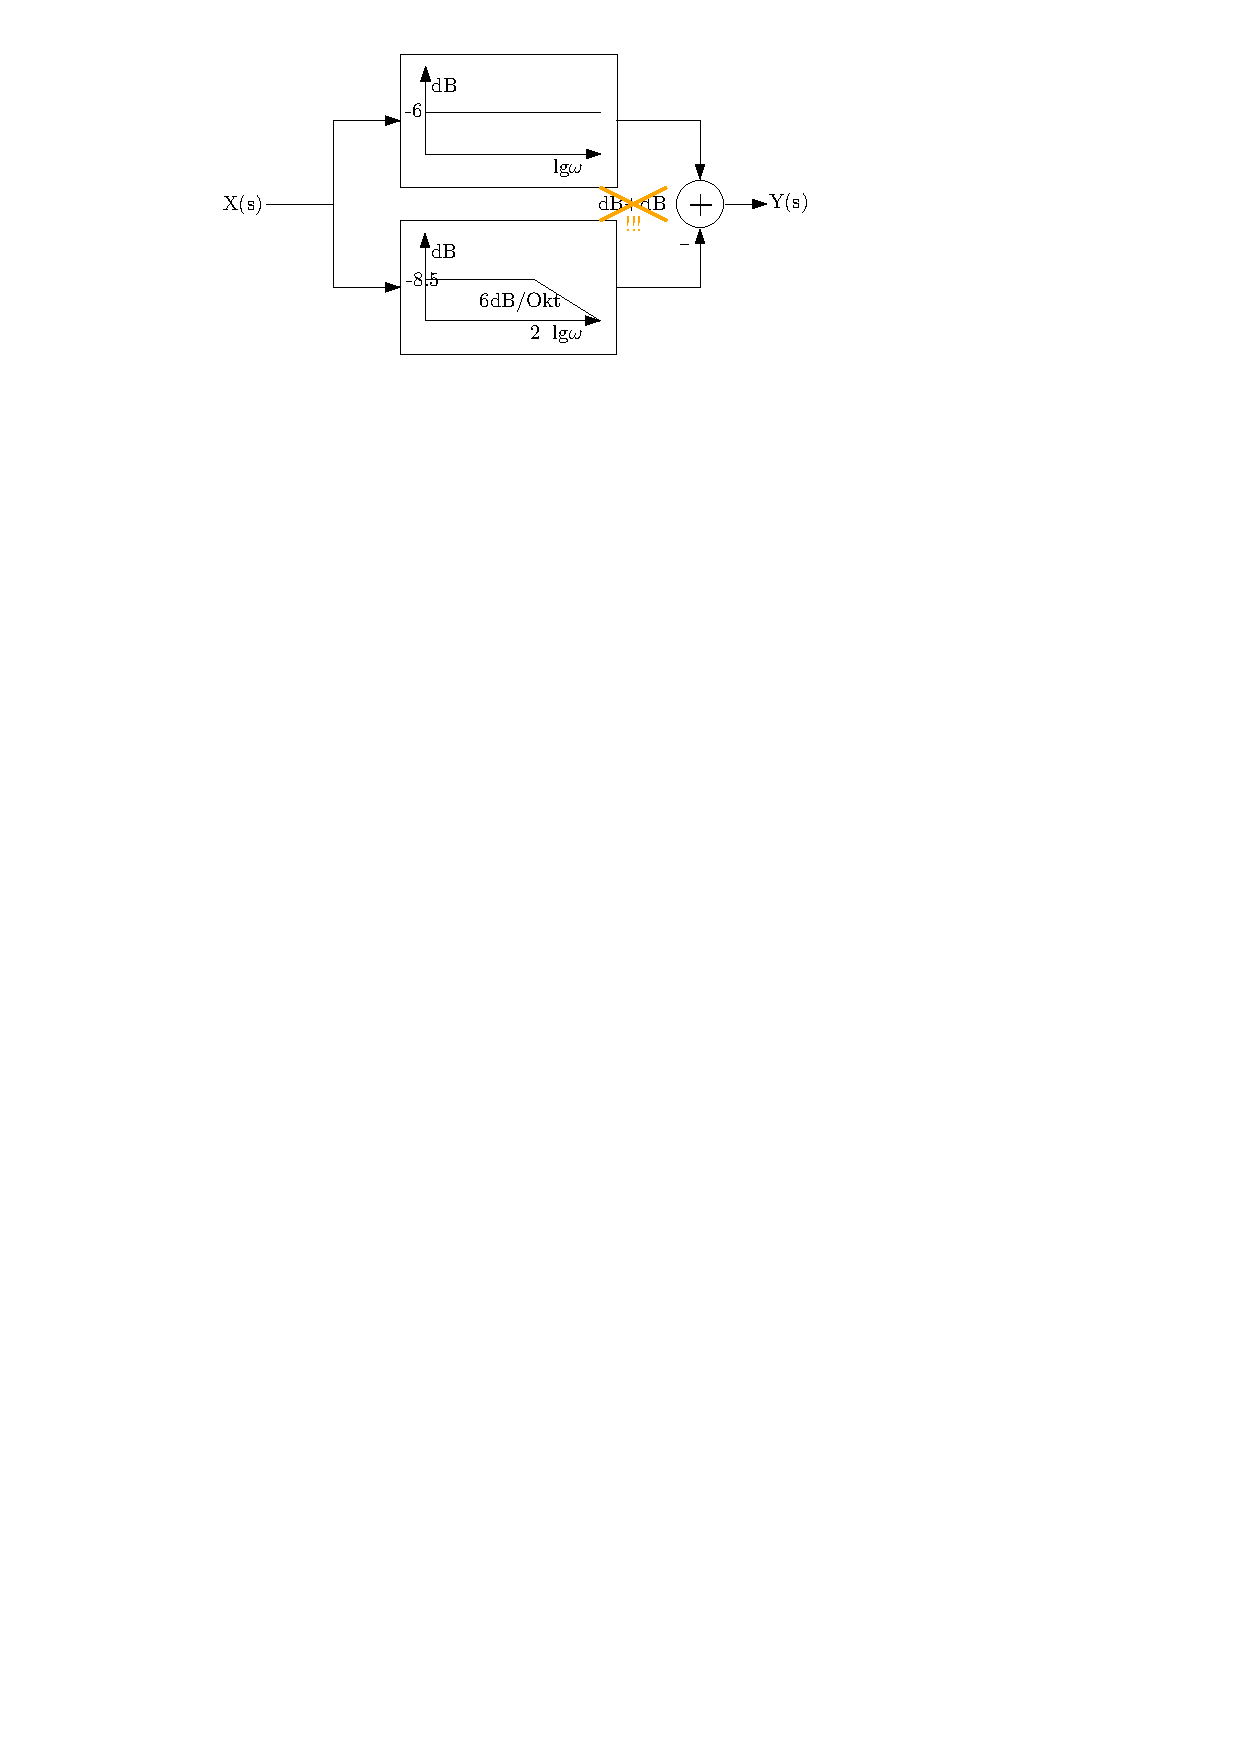
\includegraphics[width=0.59\textwidth]{../system_properties_ct/parallel_081294E23C.png}
\caption{Parallelschaltung für Aufgabe \ref{sec:081294E23C}.}
\label{fig:parallel_081294E23C}
\end{figure}






\begin{figure}
\centering
\begin{tikzpicture}[scale=1]
%
\tikzstyle{filtBlock} = [draw, rectangle, minimum height=2em, minimum width=2em, anchor=center]
\tikzstyle{filtMult} = [draw, circle, inner sep=1pt, node distance=0.8cm, anchor=center]
\tikzstyle{filtBranch}=[fill=C0, shape=circle, minimum size=5pt, inner sep=0pt, anchor=center]
\tikzstyle{filtSum} = [draw, circle, inner sep=1pt,node distance=0.8cm,anchor=center]
\tikzstyle{filtBranch2}=[fill,minimum size=0.5pt,inner sep=0pt,anchor=center]
%
%
%
\begin{scope}[shift={(0,0)}]
\matrix[row sep=5mm, column sep=5mm, ampersand replacement=\&]
{ % 1x4
\node (in){$x(t)$}; \& \node(h1)[filtBlock]{$\ast h_1(t)$}; \& \node(h2)[filtBlock]{$\ast h_2(t)$}; \& \node (out){$y(t)$};\\
};
\draw[->, C0, ultra thick] (in) -- (h1) -- (h2) -- (out);
\end{scope}
%
%
%
\begin{scope}[shift={(6,0)}]
\matrix[row sep=5mm, column sep=5mm, ampersand replacement=\&]
{ % 1x4
\node (in){$X(s)$}; \& \node(h1)[filtBlock]{$\cdot H_1(s)$}; \& \node(h2)[filtBlock]{$\cdot H_2(s)$}; \& \node (out){$Y(s)$};\\
};
\draw[->, C0, ultra thick] (in) -- (h1) -- (h2) -- (out);
\end{scope}
%
%
%
\begin{scope}[shift={(0,-1.5)}]
\matrix[row sep=5mm, column sep=5mm, ampersand replacement=\&]
{ % 1x3
\node (in){$x(t)$}; \&  \node(h1h2)[filtBlock]{$\ast\,[\,h_1(t) \ast h_2(t)\,]$}; \&  \node (out){$y(t)$}; \\
};
\draw[->, C0, ultra thick] (in) -- (h1h2) -- (out);
\end{scope}
%
%
%
\begin{scope}[shift={(6,-1.5)}]
\matrix[row sep=5mm, column sep=5mm, ampersand replacement=\&]
{ % 1x3
\node (in){$X(s)$}; \&  \node(h1h2)[filtBlock]{$\cdot\,[\,H_1(s) \cdot H_2(s)\,]$}; \&  \node (out){$Y(s)$}; \\
};
\draw[->, C0, ultra thick] (in) -- (h1h2) -- (out);
\end{scope}
\end{tikzpicture}
\caption{Reihenschaltung von zwei Systemen, links Zeitbereich, rechts Bildbereich.
Assoziativitätsgesetz der Faltung
$[x(t)\ast h_1(t)]\ast h_2(t) = x(t) \ast [h_1(t)\ast h_2(t)]$
und Dualität $x(t)\ast h(t) \laplace X(s) \cdot H(s)$.
Gesamtübertragungsfunktion $H_1(s) \cdot H_2(s)$.}
\label{fig:tikz_series_081294E23C}
\end{figure}
%
%
%
\begin{figure}
\centering
\begin{tikzpicture}[scale=1]
%
\tikzstyle{filtBlock} = [draw, rectangle, minimum height=2em, minimum width=2em, anchor=center]
\tikzstyle{filtMult} = [draw, circle, inner sep=1pt, node distance=0.8cm, anchor=center]
\tikzstyle{filtBranch}=[fill=C0, shape=circle, minimum size=5pt, inner sep=0pt, anchor=center]
\tikzstyle{filtSum} = [draw, circle, inner sep=1pt,node distance=0.8cm,anchor=center]
\tikzstyle{filtBranch2}=[fill,minimum size=0.5pt,inner sep=0pt,anchor=center]
%
%
%
\begin{scope}[shift={(0,0)}]
\matrix[row sep=5mm, column sep=5mm, ampersand replacement=\&]
{ % 3x5
\&  \& \node(h1)[filtBlock]{$\ast h_1(t)$}; \& \& \\
\node (in){$x(t)$}; \& \node (split)[filtBranch]{}; \&  \& \node (join) [filtSum]{$+$};  \& \node (out){$y(t)$};\\
\&  \& \node(h2)[filtBlock]{$\ast h_2(t)$}; \& \& \\
};
\draw[-, C0, ultra thick] (in) -- (split);
\draw[->, C0, ultra thick] (split) -- (h1);
\draw[->, C0, ultra thick] (split) -- (h2);
\draw[->, C0, ultra thick] (h1) -- (join);
\draw[->, C0, ultra thick] (h2) -- (join);
\draw[->, C0, ultra thick] (join) -- (out);
\end{scope}
%
%
%
\begin{scope}[shift={(6,0)}]
\matrix[row sep=5mm, column sep=5mm, ampersand replacement=\&]
{ % 3x5
\&  \& \node(h1)[filtBlock]{$\cdot H_1(s)$}; \& \& \\
\node (in){$X(s)$}; \& \node (split)[filtBranch]{}; \&  \& \node (join) [filtSum]{$+$};  \& \node (out){$Y(s)$};\\
\&  \& \node(h2)[filtBlock]{$\cdot H_2(s)$}; \& \& \\
};
\draw[-, C0, ultra thick] (in) -- (split);
\draw[->, C0, ultra thick] (split) -- (h1);
\draw[->, C0, ultra thick] (split) -- (h2);
\draw[->, C0, ultra thick] (h1) -- (join);
\draw[->, C0, ultra thick] (h2) -- (join);
\draw[->, C0, ultra thick] (join) -- (out);
\end{scope}
%
%
%
\begin{scope}[shift={(0,-2.5)}]
\matrix[row sep=5mm, column sep=5mm, ampersand replacement=\&]
{ % 1x3
\node (in){$x(t)$}; \&  \node(h1h2)[filtBlock]{$\ast\,[\,h_1(t) + h_2(t)\,]$}; \&  \node (out){$y(t)$}; \\
};
\draw[->, C0, ultra thick] (in) -- (h1h2) -- (out);
\end{scope}
%
%
%
\begin{scope}[shift={(6,-2.5)}]
\matrix[row sep=5mm, column sep=5mm, ampersand replacement=\&]
{ % 1x3
\node (in){$X(s)$}; \&  \node(h1h2)[filtBlock]{$\cdot\,[\,H_1(s) + H_2(s)\,]$}; \&  \node (out){$Y(s)$}; \\
};
\draw[->, C0, ultra thick] (in) -- (h1h2) -- (out);
\end{scope}
%
\end{tikzpicture}
\caption{Parallelschaltung von zwei Systemen, links Zeitbereich, rechts Bildbereich.
Distributivgesetz der Faltung
$[x(t)\ast h_1(t)]+[x(t) \ast h_2(t)] = x(t) \ast [h_1(t)+h_2(t)]$
und Dualität $x(t)\ast h(t) \laplace X(s) \cdot H(s)$.
Gesamtübertragungsfunktion $H_1(s) + H_2(s)$.}
\label{fig:tikz_parallel_081294E23C}
\end{figure}

















\clearpage
\subsection{Fourier Transformation eines schmalbandigen Impulses (Frequenzgruppe)}
\label{sec:8844932657}
\begin{Ziel}
Wir machen an dieser Stelle einen kleinen Rückgriff auf Übung 4, thematisch
also Fouriertransformation.
Wir wollen das Spektrum eines modulierten Gaussimpuls berechnen.
Dies wird uns als Modell eines schmalbandigen Spektrums gute
Dienste leisten.
Wir werden es in der nächsten Aufgabe zur Berechnung der sogenannten
Gruppenlaufzeit benutzen.
\end{Ziel}
\textbf{Aufgabe} {\tiny 8844932657}: Gegeben ist das Signal
\begin{align}
  x(t) = \cos(\omega_0 [t-t_0]) \cdot \e^{-\alpha^2 [t-t_0]^2}
\end{align}
für $\omega_0 = \frac{1}{10}$ rad/s und $\alpha=\nicefrac{3}{800}$, $t_0 = 600$ s,
also eine Gaussglocke moduliert mit einen Cosinusträger, beides zeitverzögert.

Zeigen Sie, dass die Korrespondenz der Fourier Transformation
\begin{align}
  &x(t) = \cos\left(\frac{1}{10} [t-600]\right) \cdot \e^{-\left(\nicefrac{3}{800}\right)^2 [t-600]^2}\\
  &\fourier\nonumber\\
  &X(\im\omega) = \frac{400}{3}\sqrt{\pi}\left(
  \e^{-\left(\frac{400}{3}\right)^2 \omega^2 + \left(-\left(\frac{400}{3\sqrt{5}}\right)^2-600\im\right)\omega - \left(\frac{40}{3}\right)^2}+
  \e^{-\left(\frac{400}{3}\right)^2 \omega^2 + \left(\left(\frac{400}{3\sqrt{5}}\right)^2-600\im\right)\omega - \left(\frac{40}{3}\right)^2}\right)
\end{align}
gilt.
Skizzieren Sie das Signal $x(t)$ und das Betragsspektrum $|X(\im\omega)|$.

%------------------------------------------------------------------------------
\begin{Werkzeug}
Siehe UE 4. Mit Korrespondenzentabelle arbeiten. Es ist ein wenig Schreibarbeit,
aber es artet noch nicht ganz so aus.
\end{Werkzeug}
\begin{Ansatz}
Empfehlenswert, da LTI: zuerst unverschobene Signale transformieren,
dann Zeitverzögerung berücksichtigen.
\end{Ansatz}
\begin{ExCalc}

%------------------------------------------------------------------------------
\noindent\textbf{Skalierung Dirac Impuls}:
\begin{align}
\delta(t) =& |a| \cdot \delta(a t)\\
\delta(t-b) = & |a| \cdot \delta(a [t-b])
\end{align}
%
\noindent\textbf{Cosinus-Signal}:
\begin{align}
&\text{Ansatz: } \cos(1 t) \quad\fourier\quad \pi\delta(\omega - 1) + \pi\delta(\omega + 1)\\
&\text{Zeitskalierung: } \cos(\frac{1}{10} t) \quad\fourier\quad 10 \pi\delta(10 \omega - 1) + 10 \pi\delta(10 \omega + 1) \\
&\text{Dirac Skalierung: } \cos(\frac{1}{10} t) \quad\fourier\quad \pi\delta(\omega - \frac{1}{10}) + \pi\delta(\omega + \frac{1}{10}) \\
&\text{Zeitverschiebung bzgl. [t-600]!: } \cos(\frac{1}{10} [t - 600]) \fourier \pi\delta(\omega - \frac{1}{10})\e^{-\im 600 \omega} + \pi\delta(\omega + \frac{1}{10})\e^{-\im 600 \omega}
%&\text{Dirac Skalierung zum Check: } \cos(\frac{1}{10} [t - 600]) \quad\fourier\quad 10\pi\delta(10\omega - 1)\e^{-\im 600 \omega} + 10\pi\delta(10\omega + 1)\e^{-\im 600 \omega} \\
%&\text{Dirac Austast: } \cos(\frac{1}{10} [t - 600]) \quad\fourier\quad \pi\delta(\omega - \frac{1}{10})\e^{-\im 60} + \pi\delta(\omega + \frac{1}{10})\e^{+\im 60} \\
%&\text{Dirac Skalierung, Wolfram Alpha ok: } \cos(\frac{1}{10} [t - 600]) \quad\fourier\quad 10\pi\delta(10\omega - 1)\e^{-\im 60} + 10\pi\delta(10\omega + 1)\e^{+\im 60}
\end{align}
%
\noindent\textbf{Gaussglocke}:
\begin{align}
&\text{Ansatz: } \alpha = \left(\nicefrac{3}{800}\right)\\
&\text{Unverschoben: } \e^{-\left(\nicefrac{3}{800}\right)^2 t^2} \fourier \sqrt{\frac{\pi}{\left(\nicefrac{3}{800}\right)^2}}
\e^{-\frac{\omega^2}{4 \left(\nicefrac{3}{800}\right)^2}}
=\sqrt{\pi} \frac{800}{3} \e^{-\left(\frac{400}{3}\right)^2 \omega^2}\\
&\text{Verschoben: } \e^{-\left(\nicefrac{3}{800}\right)^2 [t-600]^2} \fourier
=\sqrt{\pi} \frac{800}{3} \e^{-\left(\frac{400}{3}\right)^2 \omega^2} \e^{-\im 600 \omega}
\end{align}
%
\noindent\textbf{Faltung der Spektren}:
\begin{align}
\frac{1}{2\pi} \left(\pi\delta(\omega - \frac{1}{10})\e^{-\im 600 \omega} + \pi\delta(\omega + \frac{1}{10})\e^{-\im 600 \omega}\right)
\ast_\omega
\left(\sqrt{\pi} \frac{800}{3} \e^{-\left(\frac{400}{3}\right)^2 \omega^2} \e^{-\im 600 \omega}\right)
\end{align}
1. Teilintegral
\begin{align}
\sqrt{\pi} \frac{400}{3}
\delta(\omega - \frac{1}{10})\e^{-\im 600 \omega}
\ast_\omega
\e^{-\left(\frac{400}{3}\right)^2 \omega^2} \e^{-\im 600 \omega}\nonumber\\
%\end{align}
%\begin{align}
=\sqrt{\pi} \frac{400}{3} \int\limits_{\nu =-\infty}^{+\infty}
\delta(\nu - \frac{1}{10})\e^{-\im 600 \nu}
\e^{-\left(\frac{400}{3}\right)^2 (-\nu+\omega)^2} \e^{-\im 600 (-\nu+\omega)}\fsd \nu
\end{align}
mit Austasteigenschaft
\begin{align}
\sqrt{\pi} \frac{400}{3}
\e^{-\im 600 \frac{1}{10}}
\e^{-\left(\frac{400}{3}\right)^2 (-\frac{1}{10}+\omega)^2} \e^{-\im 600 (-\frac{1}{10}+\omega)}
%\end{align}
% \begin{align}
% \sqrt{\pi} \frac{400}{3}
% \e^{-\im 60}
% \e^{-\left(\frac{400}{3}\right)^2 (\frac{1}{100}-\frac{1}{5}\omega+\omega^2)} \e^{\im 60} \e^{-\im 600 \omega}
% \end{align}
% \begin{align}
% \sqrt{\pi} \frac{400}{3}
% \e^{-\left(\frac{400}{3}\right)^2 (\frac{1}{100})}
% \e^{-\left(\frac{400}{3}\right)^2 (-\frac{1}{5}\omega)}
% \e^{-\left(\frac{400}{3}\right)^2 (+\omega^2)}
%  \e^{-\im 600 \omega}
% \end{align}
%\begin{align}
=\sqrt{\pi} \frac{400}{3}
\e^{-\left(\frac{40}{3}\right)^2}
\e^{+\left(\frac{400}{3 \sqrt{5}}\right)^2 \omega}
\e^{-\left(\frac{400}{3}\right)^2 \omega^2}
 \e^{-\im 600 \omega}
\end{align}
%
%
%
2. Teilintegral
\begin{align}
\sqrt{\pi} \frac{400}{3}
\delta(\omega + \frac{1}{10})\e^{-\im 600 \omega}
\ast_\omega
\e^{-\left(\frac{400}{3}\right)^2 \omega^2} \e^{-\im 600 \omega}\nonumber\\
%\end{align}
%\begin{align}
=\sqrt{\pi} \frac{400}{3} \int\limits_{\nu =-\infty}^{+\infty}
\delta(\nu + \frac{1}{10})\e^{-\im 600 \nu}
\e^{-\left(\frac{400}{3}\right)^2 (-\nu+\omega)^2} \e^{-\im 600 (-\nu+\omega)}\fsd \nu
\end{align}
mit Austasteigenschaft
\begin{align}
\sqrt{\pi} \frac{400}{3}
\e^{-\im 600 (-\frac{1}{10})}
\e^{-\left(\frac{400}{3}\right)^2 (-(-\frac{1}{10})+\omega)^2} \e^{-\im 600 (-(-\frac{1}{10})+\omega)}
%\end{align}
% \begin{align}
% \sqrt{\pi} \frac{400}{3}
% \e^{\im 60}
% \e^{-\left(\frac{400}{3}\right)^2 (\frac{1}{10}+\omega)^2} \e^{-\im 600 (\frac{1}{10}+\omega)}
% \end{align}
% \begin{align}
% \sqrt{\pi} \frac{400}{3}
% \e^{-\left(\frac{400}{3}\right)^2 (\frac{1}{100}+\frac{1}{5}\omega+\omega^2)} \e^{-\im 600 \omega}
% \end{align}
% \begin{align}
% \sqrt{\pi} \frac{400}{3}
% \e^{-\left(\frac{400}{3}\right)^2 (\frac{1}{100})}
% \e^{-\left(\frac{400}{3}\right)^2 (\frac{1}{5}\omega)}
% \e^{-\left(\frac{400}{3}\right)^2 (\omega^2)}
% \e^{-\im 600 \omega}
% \end{align}
%\begin{align}
=
\sqrt{\pi} \frac{400}{3}
\e^{-\left(\frac{40}{3}\right)^2}
\e^{-\left(\frac{400}{3 \sqrt{5}}\right)^2 \omega}
\e^{-\left(\frac{400}{3}\right)^2 \omega^2}
\e^{-\im 600 \omega}
\end{align}


\end{ExCalc}
\begin{Loesung}
Wir sehen anhand dieses vergleichsweise einfachen Signals, dessen Parameter
didaktisch sinnvoll getuned sind, dass hinter unseren SigSys-Berechnungsvorschriften
langwierige (aber im Grunde immer noch triviale)
Rechnungen stecken können. Daher können wir heutzutage froh sein,
wenn der Rechner uns die Arbeit abnimmt.
Wir sollten allerdings ein Gefühl dafür entwickeln, welcher Aufwand hinter
einer Lösung steckt, und ob ein computer-generiertes Ergebnis stimmen
kann. Bei dem Spektrum, was wir gerade berechnet haben, kann z.B.
kein $w^3$ Term auftreten. Solche Sachen deuten dann sehr schnell auf Fehler hin.
Daher: je mehr wir per Hand durchgerechnet haben (in SigSys reichen zunächst
Systeme 1. und 2. Ordnung), desto besser können wir einem Computer beibringen, was er/sie
für uns Rechnen soll.

In \fig{fig:frequency_group_8844932657} ist das Signal (oben) und dessen
Betragsspektrum (unten) visualisiert.
%
Wir sehen, dass der Gaussimpuls mittels Cosinus zu den Frequenzeinträgen
um $\omega=\pm \frac{1}{10}$ rad/s
moduliert wurde.
Oder wieder andere Sichtweise: Die beiden Dirac Impulse im Spektren des idealen,
unendlichen Cosinus werden durch dessen zeitliche Begrenzung verschmiert
(Faltung mit der Gaussglocke).
%

Wir haben uns ein sehr feines Beispiel gebastelt, um uns nun den
Begriff einer kleinen Frequenzgruppe anschaulich zu machen.
Das Spektrum ist zwar streng genommen nicht bandbegrenzt, weil die Gaussglocke
nur asymptotisch gegen Null geht, aber die Hauptenergie des Spektrums
steckt in dem sichtbaren Gaussimpuls.
Und diese konzentriert sich \textbf{relativ} zu $\omega_0=\frac{1}{10}$ rad/s in einem
\textbf{kleinen Frequenzbereich}. Dies wird gerne \textbf{Frequenzgruppe} genannt.
Hinweis: eine noch kleinere (unendlich schmal) Frequenzgruppe wäre im Sinne der
Mathematik noch eleganter, aber dann sehen wir in den Grafiken nicht mehr die
wesentlichen Dinge.
\end{Loesung}

\begin{figure}[h]
\centering
\includegraphics[width=1\textwidth]{../system_properties_ct/frequency_group_8844932657.pdf}
\caption{Aufgabe \ref{fig:frequency_group_8844932657}. \texttt{frequency\_group\_8844932657.ipynb}.}
\label{fig:frequency_group_8844932657}
\end{figure}


% \begin{align}
%   &x(t) = \cos(\omega_0 [t]) \cdot \e^{-\alpha^2 [t]^2}
%   \fourier
%   X(\im\omega) = \frac{1}{2\pi} \left([\pi\delta(\omega+\omega_0)+\pi\delta(\omega-\omega_0)]\ast\sqrt{\frac{\pi}{\alpha^2}}\e^{-\frac{\omega^2}{4\alpha^2}}\right)\\
%   &x(t) = \cos(\omega_0 [t-\tau]) \cdot \e^{-\alpha^2 [t-\tau]^2}
%   \fourier
%   X(\im\omega) = \frac{1}{2\pi} \left([\pi\delta(\omega+\omega_0)+\pi\delta(\omega-\omega_0)]\ast\sqrt{\frac{\pi}{\alpha^2}}\e^{-\frac{\omega^2}{4\alpha^2}}\right) \e^{-\im \omega \tau}
% \end{align}
% Mit Zahlen
% \begin{align}
%   &x(t) = \cos(\frac{1}{10} [t-600]) \cdot \e^{-(\nicefrac{3}{800})^2 [t-600]^2}
%   \fourier
%   X(\im\omega) = \frac{1}{2\pi} \left([\pi\delta(\omega+\frac{1}{10})+\pi\delta(\omega-\frac{1}{10})]\ast\sqrt{\frac{\pi}{(\nicefrac{3}{800})^2}}\e^{-\frac{\omega^2}{4(\nicefrac{3}{800})^2}}\right) \e^{-\im \omega 600}
% \end{align}
% vereinfacht
% \begin{align}
%   &x(t) = \cos(\frac{1}{10} [t-600]) \cdot \e^{-(\nicefrac{3}{800})^2 [t-600]^2}
%   \fourier
%   X(\im\omega) = \left([\delta(\omega+\frac{1}{10})+\delta(\omega-\frac{1}{10})]\ast\sqrt{\pi}\frac{400}{3}\e^{-\omega^2(\nicefrac{400}{3})^2}\right) \e^{-\im \omega 600}
% \end{align}
% Austast
% \begin{align}
%   &x(t) = \cos(\frac{1}{10} [t-600]) \cdot \e^{-(\nicefrac{3}{800})^2 [t-600]^2}
%   \fourier
%   X(\im\omega) = \sqrt{\pi}\frac{400}{3}\left(\e^{-[\omega+\frac{1}{10}]^2(\nicefrac{400}{3})^2}+\e^{-[\omega-\frac{1}{10}]^2(\nicefrac{400}{3})^2}\right) \e^{-\im \omega 600}
% \end{align}
% \begin{align}
%   &x(t) = \cos\left(\frac{1}{10} [t-600]\right) \cdot \e^{-\left(\nicefrac{3}{800}\right)^2 [t-600]^2}\\
%   &\fourier\\
%   &X(\im\omega) = \frac{400}{3}\sqrt{\pi}\left(
%   \e^{-\left(\frac{400}{3}\right)^2 \omega^2 + \left(-\left(\frac{400}{3\sqrt{5}}\right)^2-600\im\right)\omega - \left(\frac{40}{3}\right)^2}+
%   \e^{-\left(\frac{400}{3}\right)^2 \omega^2 + \left(\left(\frac{400}{3\sqrt{5}}\right)^2-600\im\right)\omega - \left(\frac{40}{3}\right)^2}\right)
% \end{align}


\clearpage
\subsection{Phasenfrequenzgang und Gruppenlaufzeit}
\label{sec:AB91F8317C}
\begin{Ziel}
Wir wollen uns den Phasenfrequenzgang und die sogenannte Gruppenlaufzeit
genauer anschauen. Neben der Beurteilung des Pegels über die Frequenz,
also wie selektiv ein System Signale mit bestimmten Frequenzen und/oder
Frequenzgruppen durchlässt, ist auch die Phasenlage dieser Frequenzen und/oder
-gruppen von entscheidender Bedeutung, weil sie mitbestimmt, wie ein Eingangssignal
zeitlich 'verschliffen' wird.
Wir werden uns das wieder mit einem einfachen Beispiel der hier eingeführten
Systeme und Signale erarbeiten.
\end{Ziel}
\textbf{Aufgabe} {\tiny AB91F8317C}:

\noindent I. Berechnen Sie die Gruppenlaufzeit
der in Aufgabe \ref{sec:E1E7E53CFF} gegebenen Systeme und
tragen Sie diese zusammen mit dem Phasenfrequenzgang über die Kreisfrequenz auf.

\noindent II. Interpretieren Sie die \fig{fig:envelope_AB91F8317C}. Diese Grafiken
zeigen das Eingangssignal aus Aufgabe \ref{sec:8844932657} und die um den
Betragsfrequenzgang kompensierten Ausgangssignale der drei betrachteten
Systeme.

\begin{Werkzeug}
\begin{align}
\text{Gruppenlaufzeit (group delay)}
\qquad&\tau_\mathrm{GD}(\omega) = -\frac{\fsd}{\fsd \omega} \angle H(\im\omega)\\
\text{Phasenlaufzeit (phase delay)}
\qquad&\tau_\mathrm{PD}(\omega) = -\frac{\angle H(\im\omega)}{\omega}
\end{align}
\end{Werkzeug}
\begin{Ansatz}
I. Wir brauchen für den Phasenfrequenzgang die
Phase von $H(s)\bigg|_{s=\im\omega}$, also die Funktion $\angle H(\im\omega)$.
Die Gruppenlaufzeit $\tau_\mathrm{GD}(\omega)$ als Funktion über $\omega$
berechnet sich dann gemäß der Berechnungsvorschrift aus der negativen Ableitung
der Phase nach der Kreisfrequenz.
Wir haben beides bereits in Aufgabe \ref{sec:E1E7E53CFF} für alle drei
Systeme berechnet.
\end{Ansatz}
%\begin{ExCalc}
%\end{ExCalc}
\begin{Loesung}
\textbf{Teilaufgabe I}: Wir sehen, dass die vergleichsweise einfachen Systeme
schon relativ  komplizierte Funktionen hervorbringen, die wir nach den Regeln der
Kurvendiskussion (vor allem Max-/Minima, Wendepunkte) analysieren könnten.
%
\begin{align}
&\angle H(\im\omega)_\mathrm{max} =
\mathrm{atan}\left(\frac{20}{8\omega-\frac{8}{\omega}}\right)\text{in rad}
&-\frac{\fsd}{\fsd \omega} \angle H(\im\omega)_\mathrm{max}=
\frac{10(\omega^2+1)}{4\omega^4+17\omega^2+4}\text{in s}
\\
&\angle H(\im\omega)_\mathrm{min} =
\mathrm{atan}\left(\frac{-12}{8\omega+\frac{8}{\omega}}\right)\text{in rad}
&-\frac{\fsd}{\fsd \omega} \angle H(\im\omega)_\mathrm{min}=
\frac{-6(\omega^2-1)}{4\omega^4+17\omega^2+4}\text{in s}
\\
&\angle H(\im\omega)_\mathrm{all} =
\mathrm{atan}\left(\frac{4}{\omega-\frac{4}{\omega}}\right)\text{in rad}
&-\frac{\fsd}{\fsd \omega} \angle H(\im\omega)_\mathrm{all}=
\frac{4}{\omega^2+4}\text{in s}
\end{align}
%

Wir begnügen uns an dieser Stelle damit, die Funktionen von einem Computer zeichnen
zu lassen, aber nicht ohne zumindest die markanten Frequenzen $\omega\to 0$,
$\omega\to \infty$ und für die speziellen Systeme $\omega = 1$ zu checken, siehe
Aufgabe \ref{sec:E1E7E53CFF}. Dann haben wir für die Grafiken eine
bessere Erwartungshaltung.
%
Für Teilaufgabe I sind nun in
\fig{fig:group_delay_AB91F8317C} der Phasenfrequenzgang
und die Gruppenlaufzeit über die logarithmische Kreisfrequenz aufgetragen.
%
Was können wir aus den Grafiken herauslesen?

Erinnern wir uns an Aufgabe 3.4,
das RC Glied, als Tiefpass 1. Ordnung, das sogenannte PT1-Glied.
Dort hatten wir für eine spezielle Frequenz, die Grenzfrequenz des Systems
den eingeschwungenen Zustand ausgerechnet und den typischen 45 Grad Phasenversatz
zwischen Ausgangs- und Eingangssignal wiedergefunden (genau genommen: der Ausgang
folgt dem Eingang um 45 Grad verzögert). Damals hatten wir uns das nur für
eine Frequenz angeschaut und kannten das Konzept des Phasenfrequenzgangs noch
nicht. Daher konnten wir mit dem einzelnen Phasen-Offset auch nicht genau sagen,
wie die absolute Phasenlage ist. Wir hatten daher die relativ Phasenverschiebung
als Konstrukt eingeführt. Das ist für die Wechselstromtechnik immer noch
ein valides Konstrukt.

Mit unseren SigSys Werkzeugen können wir nun aber eine viel genauere Aussage zur
Phasenlage machen, wir können nämlich auf die \textbf{absolute Phasenverschiebung}
für eingeschwungene Zustände zurückschließen, wenn wir nur den
kompletten Phasenfrequenzgang, also die Funktion Phase über die Frequenz kennen.
Diese ist für praktische Systeme immer stetig und wird bei $\omega=0$ immer mit
$k \cdot 180^\circ$, $k\in\mathbb{R}$ sein. Für gerade $k$ ist die Polarität
des Ausgangssignals gleich der des Eingangssignals. Für ungerade $k$ ist die
Polarität des Ausgangssignals invertiert.
Wir können uns das anhand $\cos(\omega t - \pi) = -\cos(\omega t)$ und $\omega\to 0$
klarmachen. Die Funktion bleibt stetig beim Übergang von $\omega\to 0$ zu $\omega=0$.
Phasenfrequenzgang für $\omega\to 0$ codiert also den Polaritätsunterschied
zwischen Ausgang und Eingang, für $\omega=0$ heisst das nichts anderes als
positiver oder negativer Gleichanteil, falls der Betrag bei $\omega=0$
ungleich Null ist.

Nun müssen wir uns klarmachen, dass nach unserer Konvention (d.h. mit der Wahl der
Vorzeichen in $\e^{\pm \im \omega t}$ in der Fouriertransformation),
positiver Phasenwert ein voreilendes Ausgangssignal und negativer Phasenwert
ein nacheilendes Ausgangssignal (weil zeitliche Verzögerung) bedeutet.

Mit diesen Informationen können wir den \textbf{Phasenfrequenzgang} in
\fig{fig:group_delay_AB91F8317C} oben nun \textbf{deuten}. Wichtig ist dafür zunächst,
in Gedanken nur ein harmonisches Signal zu berücksichtigen.
Und wir können es nicht oft genug betonen: wir schauen uns den eingeschwungenen
Zustand an.

Das maximalphasige System und der Allpass invertieren hier die Polarität, das
minimalphasige System ändert nicht die Polarität.

Für Frequenzen $\omega\ll 0.1$ rad/s und $\omega\gg 10$ rad/s gibt es
beim minimalphasigen System keine Phasenverschiebung zwischen Aus- und Eingangssignal.
Im Bereich $0.1 < \omega < 10$~rad/s resultiert beim minimalphasigen System
ein nacheilendes Ausgangssignal,
mit einer maximalen Verzögerung bei exakt $\omega=1$ rad/s um ca. $37^\circ$.
Bemerkenswert ist, dass dieser Phasengang über logarithmische Frequenz Axialsymmetrie
bzgl. $\omega=1$ aufweist. Das ist zufällig nützlich für das menschliche Hören.
Es ist sehr unwahrscheinlich (aber auch nicht ausschließbar),
dass sich das menschliche Gehör in der Evolution an SigSys-Eigenschaften
orientiert hat, daher dürfen wir uns da mal wundern und freuen gleichzeitig.

Das maximalphasige System liefert voreilende Ausgangssignale (um genau die Hälfte
der Periodendauer, diese Info liefert uns die Phasenlaufzeit) für ca.
$\omega<0.1$ rad/s. Keine Verzögerung für ca. $\omega>10$ rad/s.
In dem Bereich $0.1 < \omega < 10$ rad/s ist die Phase fallend.
Bei der markanten Frequenz $\omega=1$ rad/s ist die Phase exakt $90^\circ$, d.h.
voreilend, d.h. $\cos(t+\frac{\pi}{2})\to -\sin(t)$.

Der Allpass verhält sich ähnlich wie das maximalphasige System, der abfallende
Verlauf erfolgt jedoch erst eine Oktave später, so dass sich für
$\omega=2$ rad/s die Phase $90^\circ$ findet. Es handelt sich jedoch nicht um eine
reine Verschiebung des maximalphasigen Phasenfrequenzgangs!!

Nun zur \textbf{Deutung der Gruppenlaufzeit Teilaufgabe II}:
%Ohne diese konkret zu berechnen, können wir uns die Folgen einer negative
%Ableitung der Phase nach der Kreisfrequenz klarmachen. Der Logarithmus
%streckt bzw. staucht den Funktionsverlauf, aber nicht deren prinzipielles
%Aussehen.

Um die Idee der Gruppenlaufzeit zu verinnerlichen, müssen wir das Konzept des
eingeschwungenen Zustands ein wenig aufweichen und das eher trockener
anhand der Fouriertransformation einer Frequenzgruppe diskutieren, also
$y(t) = x(t)\ast h(t)\fourier Y(\im\omega)=X(\im\omega)\cdot H(\im\omega)$
bemühen. Dafür hatten wir in Aufgabe \ref{sec:8844932657} das Signal $x(t)$
designed, welches wir nun durch die drei Systeme schicken.

Wenn wir bei den Ausgangssignalen dann die Systemverstärkung oder -dämpfung
kompensieren, sehen wir bei gleichzeitiger Darstellung von Ein- und Ausgangssignal
über die Zeit die Phasenlaufzeit aus den Signalen selber und die \textbf{Gruppenlaufzeit}
aus den sogenannten \textbf{Einhüllenden} der Signale.
In unserem Beispiel ist die Einhüllende die
Gaussglocke mit der wir das Eingangssignal mit $\omega_0=0.1$ rad/s erzeugt hatten.

In \fig{fig:envelope_AB91F8317C} ist oben das maximalphasige System, in
der Mitte das minimalphasige System und unten der Allpass dargestellt. In blau
der Eingangsimpuls und die Einhüllende davon, in orange das Ausgangssignal
und dessen Einhüllende.

Wir sehen deutlich die unterschiedlichen Phasenlaufzeiten. Bei $\omega_0=0.1$ rad/s
haben wir bei eingeschwungenen Zustand annähernd 180 Grad Phasenverschiebung
beim Maximalphasensystem und beim Allpass, was sich in dem Phasenunterschied
des Cosinusträgers äußert (es ist kein exakter Polaritätswechsel, da nicht exakt
180 Grad). Für das minimalphasige System durchläuft ein Signal mit
$\omega_0=0.1$ rad/s fast keine Phasenverschiebung, daher liegen Aus- und Eingangsimpulse
fast übereinander.

Die Verzögerung (oder das Voreilen)
der Einhüllenden des Ausgangssignals im Vergleich zur Einhüllenden des
Eingangssignals ist nun die sogenannte Gruppenlaufzeit für die betrachtete
Frequenzgruppe. Das ist in der untenstehenden Prinzip-Grafik ersichtlich.
\begin{center}
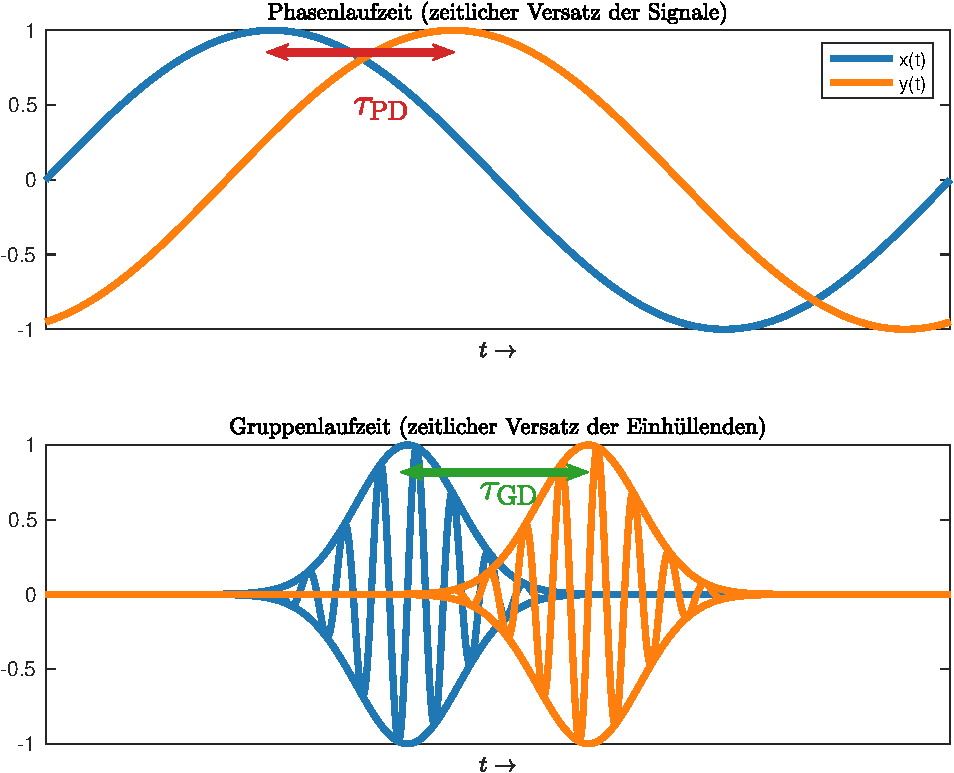
\includegraphics[width=0.5\textwidth]{../system_properties_ct/PhasenGruppenlaufzeit.pdf}
\end{center}
Die Gruppenlaufzeit ist also die Zeit die zwischen den beiden Einhüllenden
einer infinitesimalen Frequenzgruppe liegt. Wenn wir das für alle 'Frequenzgruppen'
$\fsd w$ über $\omega$ machen, bekommen wir die Gruppenlaufzeit als Funktion
über die Kreisfrequenz.

In unserer Grafik ist ein Bereich von 1200 s dargestellt, die Gruppenlaufzeit
für die Frequenzgruppe bei $\omega_0=0.1$ rad/s beträgt zwischen 1 s und 2.5 s, je
nach System. Daher ist der Offset zwischen den Einhüllenden nicht sichtbar
und als Text angegeben.
Um die Grafik zu erstellen, wurde ein zeitdiskretes Filter und Signal entworfen,
was den zeitkontinuierlichen Fall praxisnah annähert. Daher kommen die
leichten Abweichungen zur analytischen Lösung, diese Abweichungen könnten wir
noch kleiner machen, dann aber einhergehend mit höherem Computer-Rechenaufwand,
der hier gespart werden sollte.

Hinzu kommt aber noch, dass unsere erzeugte Frequenzgruppe eine praktische
Annäherung einer infinitesimalen Frequenzgruppe $\fsd \omega$ ist, was naturgemäß
Abweichungen vom analytischen Ergebnis erzeugt.

Wir sehen aber, dass die Gruppenlaufzeiten bei der Frequenzgruppe
$\omega=0.1$ rad/s aus \fig{fig:group_delay_AB91F8317C} in
\fig{fig:envelope_AB91F8317C} als Textangabe wiederzufinden sind.
\end{Loesung}
 
\begin{mdframed}
\textbf{Was bedeutet min-/maximalphasig?}
Dies ist ein Punkt den wir leider nicht im Detail analytisch anschauen können
(dafür seien \cite{LangeSigSys1, Fliege1991} empfohlen), der aber vom Wesen sehr
wichtig ist.

Wenn wir einen Betragsfrequenzgang mit exakt dem Phasenfrequenzgang
mit geringstmöglicher Phasenverschiebung verknüpfen, ist dies ein minimalphasiges
System. Es hat die geringstmögliche Gruppenlaufzeit für alle Frequenzgruppen.

Wenn wir einen Betragsfrequenzgang mit exakt dem Phasenfrequenzgang
mit maximal möglicher Phasenverschiebung verknüpfen, ist dies ein maximalphasiges
System. Es hat die größtmögliche Gruppenlaufzeit für alle Frequenzgruppen.

Wir haben z.B. ein System 1. Ordnung, können also nur einen reellen Pol und
eine reelle Nullstelle platzieren. Ein kausales System fordert den Pol in der linken
$s$-Halbebene. Je nach Pol, Nullstellenlage resultiert ein Betragsfrequenzgang,
was wir als Pegel Bode Diagramm darstellen können.
Es existiert nun ein System, was Frequenzgruppen so schnell wie möglich durchlässt
(noch schneller kann das System nicht), das ist das minimalphasige System.
Ein anderes System (es gibt hier nur die beiden Möglichkeiten, bei Systemen
höherer Ordnung gibt es dann gemischtphasige Möglichkeiten)
verzögert die Frequenzgruppen so lange wie es mit einem Pol und einer
Nullstelle eben geht (noch langsamer kann das System nicht), das ist das maximalphasige
System.
Das können wir uns auch nochmal in \fig{fig:MaxMinPhaseAllpass_numpy_E1E7E53CFF}
verdeutlichen.

\end{mdframed}


\begin{figure}[h]
\centering
\includegraphics[width=\textwidth]{../system_properties_ct/group_delay_AB91F8317C.pdf}
\caption{Phasenfrequenzgang und Gruppenlaufzeit für Aufgabe \ref{sec:AB91F8317C}.
\texttt{groupdelay\_AB91F8317C.ipynb}.}
\label{fig:group_delay_AB91F8317C}
\end{figure}
%
%
%
\begin{figure}[h]
\centering
\includegraphics[width=1\textwidth]{../system_properties_ct/envelope_AB91F8317C.pdf}
\caption{Signale und Signaleinhüllende für Aufgabe \ref{sec:AB91F8317C}.
\texttt{groupdelay\_AB91F8317C.ipynb}.}
\label{fig:envelope_AB91F8317C}
\end{figure}
